\documentclass[12pt,letterpaper]{article}
\usepackage{textcomp}

% front matter
\usepackage[latin1]{inputenc}
% \usepackage{lmodern} % keep or kill this??  might affect italics.
\usepackage{setspace}
\usepackage{amsmath}
\usepackage{amsthm}
\usepackage{amsfonts}
\usepackage{longtable}
\addtolength{\textwidth}{5cm}
\addtolength{\textheight}{5cm}
\usepackage{fullpage}
\usepackage{amssymb}
\usepackage[colorlinks=true]{hyperref}
\usepackage{url}
\usepackage{graphicx}
\usepackage{epstopdf}
\usepackage{multirow}
\usepackage{array}
\usepackage{harvard}
\usepackage{tabularx}
\citationmode{abbr}

\usepackage{float}
% \usepackage{perpage}
% \MakeSorted{figure}
% \MakeSorted{table}
\usepackage{lscape}
\usepackage{verbatim}
\usepackage{pdflscape}
\usepackage{chngcntr}
\usepackage{appendix}
\usepackage{booktabs,calc}
\usepackage{ulem}

% allow yellow highlighting in tables
\usepackage{color,colortbl}
\usepackage{soul}
\definecolor{Yellow}{rgb}{.88,1,.65}
\definecolor{Green}{rgb}{.65,1,.65}
\definecolor{Red}{rgb}{1,.65,.65}

\citationstyle{dcu}

\usepackage[labelfont=bf,center,large,labelsep=newline]{caption}
\usepackage{subfig}
% \counterwithout{subtable}{table}
\def\changemargin#1#2{\list{}{\rightmargin#2\leftmargin#1}\item[]}
\let\endchangemargin=\endlist

% define subscript / superscript commands
\newcommand{\superscript}[1]{\ensuremath{^{\textrm{#1}}}}
\newcommand{\subscript}[1]{\ensuremath{_{\textrm{#1}}}}

% create a shortcut for newlines in captions:
\newcommand{\cnewline}{\hspace{\linewidth}}

%format paper to save trees
\usepackage[right=1in,left=1in,top=1in,bottom=1in]{geometry}
\usepackage{savetrees}

%AER style headers
\def\thesection{\arabic{section}}
\def\thesubsection {\thesection.\arabic{subsection}}

% set home path
\newcommand{\HOME}{\string~}


% set paths
\newcommand{miningpath}{.}

% add Rick's formatting
\usepackage[right=1in,left=1in,top=1in,bottom=1in]{geometry}
\usepackage[all=normal,title,sections]{savetrees}
\def\thesection{\Roman{section}}
\def\thesubsection {\thesection.\Alph{subsection}}
\usepackage{changepage}

% disable hyperlinks (which are broken for appendix tables)
\usepackage[options]{nohyperref}

%allow multiple table pages
\setcounter{bottomnumber}{3}
\setcounter{topnumber}{2}
\setcounter{totalnumber}{5}
\renewcommand{\textfraction}{.001}

\title{ Rent-Seeking and Criminal Politicians: \\ Evidence from Mining
  Booms \footnote{We are thankful for useful discussions with Alberto
    Alesina, Josh Angrist, Lorenzo Casaburi, Shawn Cole, Taryn
    Dinkelman, Jim Feyrer, Claudio Ferraz, Ray Fisman, Ed Glaeser,
    Ricardo Hausmann, Richard Hornbeck, Lakshmi Iyer, Devesh Kapur,
    Asim Khwaja, Michael Kremer, Erzo Luttmer, Sendhil Mullainathan,
    Rohini Pande, Andrei Shleifer, Konstantin Sonin, Milan Vaishnav,
    Tony Venables and David Yanagizawa-Drott. We thank
    Ray Fisman and Oliver Vanden Eynde for sharing data.  Srinivas Balasubramanian,
    Alison Campion, Phoebe Liang, Kat Nicholson and Taewan Roh provided excellent
    research assistance.  This project received financial support from
    the Center for International Development and the Warburg Fund
    (Harvard University). An earlier version of this paper circulated
    with the title, ``Dirty Politics: Mining Booms and Politician
    Behavior in India.'' All errors are our own.}}

\author{Sam Asher \\ Johns Hopkins SAIS\footnote{sasher2@jhu.edu}\\ \\ Paul
  Novosad\\Dartmouth College\footnote{paul.novosad@dartmouth.edu}\\ \\ }

\begin{document}

\date{This version: May 2021\\First version: March 2013}                      

\maketitle
% \addtocounter{page}{-1}
\thispagestyle{empty}
\begin{abstract}
\doublespacing

  We study how natural resource rents affect the selection and behavior
of holders of public office. Using global price shocks to thirty-one
minerals and nationwide geological and political data from India, we
show that local mineral rent shocks cause the election of politicians
charged with serious crimes.  We also find a moral hazard effect:
politicians commit more crimes and accumulate greater wealth when
mineral prices rise during their terms in office. These politicians
have direct influence over mining operations but no access to fiscal
windfalls from mining; we thus isolate the direct political impacts of
mining sector operations.





  JEL Codes: D72, P16, O13, Q33

\end{abstract}

\newpage
% \setcounter{page}{1}
\singlespacing

\begin{QUOTE}
  ``Vested interests are controlling the whole industry. Imagine, in one night, nearly a thousand vehicles go without proper permit to a port and export the iron ore without proper permit. All this is supervised by the forest department, by the mining department, by the police, by the road transport department [...] There is a checkpost everywhere, but nobody stops them. At the port, you have to show the port security valid documents, here too they don't do anything at all. Then there are forest officers inside the port, who are supposed to check whether these minerals are from the forest area, whether they have taken permission from the forest department or not. [...] Then there is the customs department which has to collect the customs duty. Nobody does anything.''
\end{QUOTE}
\begin{flushright} \small{Justice Nitte Santosh Hegde, Former Supreme Court Judge}
\end{flushright}

\doublespacing

\section{Introduction}
\label{sec:intro}

The selection of honest politicians and the prevention of misuse
of power in office are central to good governance, especially in
developing countries where institutions place fewer constraints on the
behavior of officials \cite{Caselli2004,Besley2011a,DalBo2017}. An
important hypothesis in the literature on governance is that certain
types of economic activity directly affect who obtains power and how
they behave in office.\footnote{See, for example,
  \citeasnoun{Sokoloff2000}, \citeasnoun{Easterly2003}, and
  \citeasnoun{Acemoglu2009a}.}  The mining sector is
thought to be particularly pernicious to political institutions for
two reasons. First, it creates fiscal windfalls with no basis in
taxation, which may limit the accountability of politicians. Second,
due to the inherent nature of its operations, mining concentrates
large rents in firms, which raises the return to rent-seeking by
politicians. It has thus far proved difficult to empirically
distinguish between these two channels, which have substantially
different policy implications. In this paper, we use exogenous
variation in mineral rents, holding constant institutions and fiscal
windfalls, to isolate the impact of local mineral extraction on
politician selection and behavior.\footnote{At the country level,
  natural resource wealth is associated with worse economic and
  political outcomes in countries with weak institutions
  \cite{Mehlum2006,Arezki2011,Arezki2012,Bhattacharyya2010,Lei2014,Caselli2011}. A
  second generation of research on the subject addresses the
  endogeneity of resource-rich places by exploiting resource
  discoveries, price shocks or rent allocation formulas
  \cite{Bruckner2012,Carreri2014,Caselli2011}. For a thorough review
  of studies on the relationship between political outcomes and
  resource wealth, see \citeasnoun{Ross2015a} and
  \citeasnoun{van2010natural}.}

To generate exogenous shocks to local mineral wealth, we draw on
changes in the global prices of 31 subsurface minerals, located in
geological deposits throughout India. For a concrete example, consider
two mineral-rich areas, one of which is rich in gold, and the other
rich in silver. When the global price of gold rises relative to
silver, there is an exogenous mineral rent shock to the gold-rich
region that is not expected to be correlated with other events in that
region, except through the increased value of gold. We exclude areas
with no minerals, to avoid comparing mineral-rich to mineral-poor
areas, which may be different on many dimensions.\footnote{Our use of
  global price shocks to identify exogenous changes in mineral wealth
  is similar to \citeasnoun{Dube2013}, \citeasnoun{Bruckner2010} and
  \citeasnoun{Berman2017}, among others.}  Mandated public disclosures
allow us to observe the criminal charges filed against each candidate
contesting state-level elections in India, along with their assets.

We document three primary findings. First, increases in local mineral
rents cause criminal politicians to win more elections, in spite of
marginal increases in electoral competition.\footnote{Following
  standard practice in India, we describe candidates facing formal
  criminal charges as ``criminal politicians.'' The vast majority of
  these cases drag on for years, such that few have been resolved,
  making it impossible to conduct a similar analysis using
  convictions. We discuss the possibility that charges misrepresent
  actual crimes in Section~\ref{ssec:politics}.} The effect is
particularly large for politicians charged with violent crimes.
Second, when the value of local minerals rises during the electoral
term, elected politicians accumulate additional criminal
charges. Third, elected politicians gain substantial wealth during
mining booms.  The increases in crime and wealth are limited to
politicians who are in office; we find neither effect on politicians who
competed for office but were not elected.

Our basic specification studies the effect of a constituency-level
mineral wealth shock driven entirely by changes in the global price of
the basket of minerals produced in that constituency. To measure
adverse selection, we examine the effect of the change in mineral
wealth over the five years before an election on the likelihood that a
criminal politician gains office. To measure moral hazard, we examine
the effect on political behavior of price shocks that raise the value
of local minerals \textit{after} a politician has been elected.  All
specifications include state--year fixed effects, thus drawing only on
variation across small constituencies within Indian states. The
selection effect estimates are robust to a specification with
constituency fixed effects that relies on changes in mineral wealth
only within the same constituency across time. Due to sample size,
this specification is not available in the moral hazard estimates,
which rely on cross-sectional variation in recent price
shocks.\footnote{A constituency fixed effect analysis would require
  three observations (hence two changes) for each constituency. While
  we have three observations for most locations, a redrawing of
  constituency boundaries at the midpoint of the sample makes it
  impossible to link places across the entire time period. However, we
  present several pieces of evidence suggesting that these price
  shocks are exogenous to constituencies, supporting a causal
  interpretation of the cross-sectional design.} These effects are
robust to excluding conflict-affected districts and do not
appear in placebo tests based on unproductive deposits or price
shocks from different years. Positive economic shocks to the
manufacturing or agricultural sectors have no effects on the same
outcomes, suggesting that our results are driven by a phenomenon
specific to the mining sector rather than a general effect of economic
activity. One limitation of the moral hazard result is that we are limited to studying incumbents who chose to run for office a second time; there may therefore be some attrition bias (56\% of winners in our sample run again), but it would have to be very large to explain the full effect.

Because of the structure of mineral taxes and royalties in India, we
can rule out the possibility that these results are driven by
increases in state revenue or larger discretionary budgets for
politicians. This is important because fiscal windfalls can have
independent adverse effects on political outcomes
\cite{Robinson2006,Brollo2009,Martinez2015}. Mineral taxes and
royalties are collected by state governments and are \textit{not}
disproportionately disbursed in the areas where mining takes
place. Local increases in economic activity associated with mining may
raise revenue at other levels of government, but do not affect the
discretionary funds available to the state legislators that we
study. To our knowledge, this is the first study to isolate the impact
of natural resource wealth on political outcomes in the absence of
fiscal windfalls. In fact, several of the best identified studies on
natural resources and political outcomes draw identification from
exogenous allocation of oil windfalls to municipalities in Brazil, and
thus test strictly for the fiscal windfall impact in isolation from
direct rent-seeking from mineral extraction operations
\cite{Caselli2011,Monteiro}.\footnote{These studies exploit a formula
  that allocates royalties to municipalities based on characteristics
  unrelated to resource extraction activities in the municipalities or
  to the hold-up powers of the mayors.  They find that fiscal
  windfalls lead to: (i) increased municipal spending with little
  impact on municipal public goods \cite{Caselli2011}; and (ii)
  increased public employment and short-term incumbency advantages
  \cite{Monteiro}. \citeasnoun{Brollo2009} study fiscal windfalls that
  occur for reasons unrelated to natural resource wealth, finding that
  they cause the election of less educated mayors and cause mayors to
  engage in more corruption.}  Our study is distinct and
complementary: the direct impact of mining operations that we isolate
is a channel that these earlier studies explicitly do not address.

This paper makes two contributions to the literature on the
relationship between natural resources and political behavior. First,
we show that mineral extraction operations have a direct adverse
effect on political outcomes, even in the absence of fiscal windfalls.
Second, we provide a distinct test for moral hazard from access to
rents while in office; this effect is also economically
meaningful. Rent-seeking opportunities that emerge once politicians
are already in office cause those politicians to gain assets and
engage in new criminal behavior.\footnote{The best empirical evidence
  to date of these channels is in \citeasnoun{Brollo2009}, who model
  the adverse selection and moral hazard effects of fiscal windfalls
  in Brazil. They provide suggestive evidence that the moral hazard
  channel is important, in that controlling for candidate education
  does not change the effect of fiscal windfalls on corruption, but
  they do not rule out selection effects. \citeasnoun{Andersen2013}
  present indirect evidence of the enrichment of leaders from oil
  booms, showing that oil shocks lead to increased tax haven bank
  deposits from autocratic oil-exporting countries. Using the same
  asset data as we do, \citeasnoun{Fisman2013} find that Indian
  politicians gain disproportionate wealth when elected to office. The
  latter two papers identify returns to political office but do not
  identify politician behavior response to changes in rent-seeking
  opportunities.} While these effects may lead to similarly bad
outcomes, they have substantially different implications; paying
closer attention to voter decision-making and the operation of
elections can mitigate the selection effect, while better monitoring
of candidates in office can mitigate moral hazard.

A key question raised by our study is what form this rent-seeking
takes. The illegal behavior of politicians could be detrimental or
beneficial to mining firms. Models of politicians and firms have
usually focused on the case where politicians extract rents by
blocking access to government services like licenses and permits
\cite{Shleifer1994}. In contrast, firms could benefit from politicians
who can facilitate illegal activities, like expanding mines beyond
license boundaries, violating environmental laws, or intimidating
journalists and activists. Empirically distinguishing between these
two scenarios is difficult given the paucity of reliable data on
either the profits or revenues of mining firms, and is beyond the
scope of this paper. However, qualitative evidence suggests that firms
and politicians often have collusive relationships
\cite{Bhowmick2011,Paul2015}, as does empirical evidence from other
sectors \cite{lehne2016}. The \textit{de facto} roles of Indian
politicians as local fixers make them well-placed to provide services
to illegal mining firms, such as enforcing illegal contracts and
intimidating whistleblowers \cite{Chopra1996,Jensenius2013a}.  The
importance of violent crimes in explaining our results is also
consistent with this interpretation. Violence-using politicians are
particularly well-suited to providing the services demanded by mining
firms; as emphasized by the literature on mafias, violent actors are
often essential to the functioning of black markets, and ethnographic evidence from India suggests that politicians play precisely this role
\cite{Gambetta1996,Bandiera2003,Berenschot2011,Skarbek2011,Chimeli2011,Vaishnav2017}.

Previous studies of criminal politicians in India have largely ignored
the fact that a large share of criminal politicians face charges of
serious violent crimes \cite{Prakash2014,Fisman2013}; our preferred
interpretation, in contrast, highlights the politician's ability to
coordinate acts of violence as central to his role. We discuss the
possible role of violence in Section~\ref{sec:disc}, and formalize
these ideas in a political agency model in the spirit of
\citeasnoun{Persson2000} in Appendix~\ref{sec:model}.  However,
empirically testing these hypotheses for the specific role of violence
in the mining sector is left to future work.

\section{Background: Mining and Politics in India}
\label{sec:bg}

\subsection{The mineral industry in India}
\label{ssec:mining}

In 2010, the mining sector in India employed 521,000 workers and
produced 2.5\% of Indian GDP from over sixty different minerals
\cite{IndianBureauofMines2011c}. This is a small share of the economy
as a whole, but the output share of the mineral sector is much higher
in the localized regions where extraction takes place.
From independence until the 1990s, Indian mines were predominantly
state-owned. Many mines were privatized in the subsequent
liberalization era. By 2010, 2229 of 2999 mines were privately owned,
representing 36\% of total production value
\cite{IndianBureauofMines2011c}. The mining sector is jointly
regulated by the federal and state governments; royalties and taxes
paid by mining corporations go directly to state and federal
governments.  

Importantly, there is no requirement for fiscal proceeds from mining
to be spent in communities affected by mines, nor is there any
indication that they are.\footnote{In 2015, India revised the Mines
  and Minerals Act to require a share of mineral royalties to be paid
  to a district development fund. Even these districts are seven times
  the size of constituencies, the unit of observation in this study,
  and no such payments had yet been made in the sample period.}
Elected politicians in many states receive development funds under the
MLA Local Area Development fund schemes; these sums are small and
constant across constituencies and are thus not affected by local
mineral rents. Local taxation operates at jurisdictional levels with
no direct relationship with the legislative assemblies that are the
subject of this study. Therefore, even if mineral wealth shocks
increase local business activity, they will not affect the
discretionary budget of the local state legislator.  We can thus rule
out the possibility that our results are caused by the fiscal
windfalls present in other studies of natural resource wealth.

Large scale criminal activity was present in the mining sector
throughout the period of our study (2003--2017). Most of the illegal
activity in this period was directly linked to the role of government
in the mineral sector; management of fiscal windfalls played little
role, as royalties are treated as general funds by state and federal
governments and are not linked to mining activities. Illegal mining
includes but is not limited to: (i) underreporting of mineral output
to avoid taxes and royalties; (ii) conducting prospecting and mining
in areas without official permits, including preservation areas; (iii)
violation of environmental regulations; and (iv) bribe-taking by state
officials in exchange for mining permits. Intimidation of activists
and journalists have also been widely reported. Major mines in India
are now largely open caste mines with activities visible from outer
space, which makes illegal mining difficult to hide. Authorities are
thus virtually always complicit in illegal mining.

In 2010, the federal government formed the Shah Commission of Inquiry
to investigate illegal mining in a range of states and minerals. The
Commission documented illegal mining at a large scale in every mineral
and every state where it conducted investigations. The scale of
illegal activities implied coordination at many levels of
government. The findings of the Shah Commission eventually motivated
the Supreme Court of India to ban iron mining in three major states
\cite{wsj2013chat}. The Commission was terminated in 2013 by the
federal government with little explanation, though investigations
in several states had yet to begin.\footnote{For more information on
  illegal activity in the mining sector, see the various state reports
  of the Ministry of Mines Shah Commission. See also the report of the
  Karnataka Lokayukta (an anti-corruption commission) on iron ore
  mining (July 27, 2011). \citeasnoun{Chauhan2012} summarizes specific
  criminal allegations against mining firms in eleven different
  states.}

The case of the Reddy brothers in Karnataka encapsulates many features
of the relationship between mining and politics in India. Through
the benefit of political connections, the brothers first obtained iron
licenses in Andhra Pradesh in the early 1990s. Over the course of a
ten-year iron boom, they became key financiers of elections, eventually
becoming billionaires and government ministers. They have been charged
with a range of illegal mining activities, perhaps most brazenly of
moving the state boundary markers dividing Andhra Pradesh from
Karnataka to place their mining operations in the state with the more
favorable regulatory environment. They have openly admitted to bribing
politicians to switch parties and have been accused of various acts
of violence and intimidation \cite{Vaishnav2017}.

The mineral sector is tied to illegal behavior in many countries other
than India as well. See, for example, \citeasnoun{Africapp2013} on
illegal outflows from Africa. The very existence of an industry-funded
organization aiming in part to decreasing the amount of law-breaking
in the mining industry, the Extraction Industries Transparency
Initiative, is a case in point of the ubiquity of illegal activity in
the sector.

\subsection{Political context}
\label{ssec:politics}

Indian states have ownership rights over all minerals within their
boundaries; while federal clearances are required for the mining of
certain minerals, states have hold-up power over these as well.  State
politicians, also known as Members of Legislative Assemblies (MLAs),
are elected in first-past-the-post, single elector constituencies. The
formal powers of state politicians are exercised through the state
legislatures; while they have no formal role in the permitting
process, in practice they play a significant informal
role. A central de facto role of local politicians is to help
citizens obtain services from the state
\cite{Berenschot2011,Jensenius2013a}; they also exert significant
authority over state bureaucrats through their ability to reassign
them \cite{Iyer2012a,Vaishnav2017}. This gives local politicians
significant control over the many permits and clearances that are
required before mining operations can begin, including reconnaissance
permits, prospecting licenses, mining leases, environmental clearances
and surface rights (often to government-owned land). In other work, we
find that political factors influence the allocation of these permits
\cite{an2017pols}. The set of regulatory restrictions known as the
License Raj has persisted in the mining sector even while it was
dismantled elsewhere, and additional permits are required for the
expansion or alteration of existing leases, as well as expanding
production from given mines. The state legislator is thus one of the
most important officials that mining firms rely upon both for
facilitation of operations and for prevention of predation by the
state. We spoke with several mine operators, and each one had a
personal relationship with the legislator representing the
constituency of the mine.

From 2003--2017, 32\% of elected politicians at the state and federal
level in India were facing formal criminal charges in a court of law;
a third of these were for violent crimes (Appendix
Table~\ref{tab:pol_crimes}). Explanations for the success of criminal
politicians in India remain contested. Four prevailing hypotheses are:
(i) voters would prefer non-criminal representatives, but lack
information about the criminality of candidates
\cite{Banerjee2012b,Pande2011}; (ii) voters penalize criminal
candidates, but may nevertheless choose them for ethnic reasons
\cite{Chauchard2014a}; (iii) criminals are favored by parties because
they are self-financing \cite{Vaishnav2017};\footnote{The soaring cost
  of elections in India and tight official restrictions on spending
  lead to a high demand among politicians for untraceable money, or
  ``black money'' as it is known in India \cite{Vaishnav2017}. As an
  industry with the potential to rapidly generate undocumented cash,
  mining is widely suspected to be a significant funding source for
  many political campaigns.} and (iv) criminals are favored by voters
because they are better at delivering services from a failing state
\cite{Vaishnav2017}.

Using criminal charges as a measure of criminal behavior is subject to
the concerns that changes in reporting of crime are difficult to
distinguish from actual crime and that charges may be fabricated by
political enemies. This is a difficult problem to address and is faced
by many studies on criminal behavior by politicians in developing
countries. Most of these charges will not be resolved for decades due
to the backlog in the Indian court system; even when they are
resolved, the judgment may be politically biased
\cite{poblete2019}.

There is empirical evidence that criminally-charged politicians are
bad for their constituents, are disliked by voters, and are recognized
by parties to be weaker candidates, suggesting that the charges they
face are plausibly valid. \citeasnoun{Chemin2012} and
\citeasnoun{Prakash2014} find that average outcomes are worse in
constituencies represented by criminally-charged politicians. Vignette
studies suggest that, all things equal, voters prefer non-criminal
candidates \cite{Banerjee2012b,Chauchard2014a}, and parties are less
likely to run criminally-charged candidates in competitive elections
\cite{shaukat2018}.\footnote{See \citeasnoun{Pande2011} for a summary
  of empirical research on voter preferences for politician quality.}
Anecdotally, many politicians in fact advertise their willingness to
flout the law or ability to organize violence
\cite{Vaishnav2017}. Finally, much of our empirical focus is on
violent crimes, which are less likely to be entirely fabricated than
minor crimes \cite{iyer2012}. Henceforth, following convention in
India, we refer to criminally-charged politicians as criminal
politicians.

\section{Data}
\label{sec:data}

We combined data on electoral outcomes, candidate characteristics,
mineral deposit locations, and mineral production. India is divided
into approximately 600 districts and 4000 constituencies;
approximately 400 districts have productive mineral
deposits. Constituency and district boundaries do not cross. All of
the data is available at the constituency level, with the exception of
mineral production, which is at the district level.

Data on electoral outcomes from 1990--2017 come from the Election
Commission of India (ECI), described in \citeasnoun{Jensenius2013b}
and shared by the Trivedi Center for Political Data. We tracked
changes in names of parties over time in order to identify the local
incumbent party in each constituency.  To measure political
competition, we use the effective number of parties (ENOP), an inverse
Herfindahl measure based on vote share \cite{Laakso1979}.

Data on politician characteristics come from sworn affidavits
submitted by candidates to the ECI. These include a list of criminal
charges currently under prosecution, assets and liabilities of
candidates and their relatives, as well as the candidate's age and
education. These affidavits have been required from all candidates
seeking state-level election following Supreme Court rulings in 2002
and 2003 and have been digitized and disseminated by the Indian
Electoral Commission and the Association for Democratic Reform (ADR).
The resulting candidate-level data have been widely analyzed and
discussed in the media as well as by scholars
\cite{Prakash2014,Fisman2013}.  Election laws in India bar convicted
criminals from contesting elections; for sitting politicians, criminal
charges are the best available measure of politician
criminality. Criminal charges are unlikely to be omitted, as they are
easily verified from public record and politicians can be fined,
disqualified from elections, or imprisoned if found with incorrect
affidavits \cite{Prakash2014,Vaishnav2017}.

We computed net wealth as assets less liabilities across all family
members.\footnote{As in \citeasnoun{Fisman2013}, who study the private
  returns to political office in India, we removed candidates with net
  wealth less than Rs 100,000 (approximately USD 1500), and winsorized
  at the 1st and 99th percentile. Alternate choices do not materially
  affect the results.}  Figure \ref{fig:affidavit} shows a scan of a
submitted affidavit; the list of numbers under the entry marked (iii)
in the figure is a list of sections under the Indian Penal Code under
which this candidate has been charged.  In order to observe changes in
politician wealth and criminal behavior over time, we constructed a
time series of candidates who recontest elections.  We extended data
from \citeasnoun{Fisman2013} and ADR, manually matching candidates
based on name, age, level of education and tax ID number. We matched
50\% of winners and 34\% of runners up in our mining constituency
sample to future elections.

To verify the accuracy of the ADR-coded affidavits,
\citeasnoun{Prakash2014} re-entered all of the affidavits for the top
two candidates from 2003 to 2007. Comparing the re-entered data to the
data posted by ADR shows that fewer than 3\% of candidates changed
from criminal to non-criminal or vice versa in the recoding. However,
the number of crimes increased for about a quarter of candidates,
suggesting that the ADR data accurately identifies whether candidates
are criminally charged but underestimates the total number of
charges. We use the re-entered data where it is available and the ADR
data for the remainder of elections. Because our results focus on the
presence or absence of criminal charges, the discrepancy in the number
of charges does not affect our primary analysis. The analysis sample
includes affidavits covering the years 2003--2017.

Geocoded data on the type and size of all known mineral deposits in
India is from the Mineral Atlas of India
\cite{GeologicalSurveyofIndia2001}.\footnote{The Geological Survey of
  India is a technocratic agency which to date has remained clear of
  India's many mining scandals.  All our results except those on
  election results are from after 2001, mitigating any reverse
  causality from mineral prices to deposit discovery; the results on
  elections are robust to using data only from later dates.}
Production data are published at the district-mineral level in the
annual \textit{Statistics of Mineral Information}, which we
digitized. We divided district production into all constituencies
within a district that had matching deposits of the same mineral,
weighting by deposit sizes. 91\% of reported mineral output can be
matched to specific deposits. We defined local production as the
average value of output from 1990--2013, matching the sample of
elections to the extent possible. From a list of 45 minerals for which
we have both deposit and price data, we excluded minerals for which
the Indian Bureau of Mines does not publish production statistics (on
account of their low value), and we excluded constituencies with
economically insignificant production in all
years.\footnote{Specifically, we dropped constituencies where annual
  production never exceeded USD 100,000. The average exchange rate
  during the sample period was 45 INR per USD, but the threshold was
  established in U.S. dollars because we valued output as constituency
  production multiplied by global price.}  To account for the fact
that mineral deposits may span constituency boundaries, we also
assigned production to all constituencies within 10km of an active
deposit, using a triangular kernel that puts the greatest weight on
the nearest deposits. Results are robust to alternate choices on all
of these dimensions, many of which are shown in appendix tables.

We include both public and private mines, which are not distinguished
in any of the data sources that we use. Given the private returns to
illegal mining and the key role of politicians, both public and
private mining operations create opportunities for rent-seeking. 

Appendix Figure~\ref{fig:app_sample} shows how we construct our
analysis sample of 946 constituency elections, which covers 31
distinct mineral types across 25 Indian states. Figure
\ref{fig:deposit_map} shows a map of deposit locations, along
with district-level production, where the most productive districts
are shaded the darkest. The map reveals the wide dispersion of
minerals across India. Most of the unexploited deposits are in the
difficult-to-access Himalaya mountain region.

Commodity prices come from the United States Geological Survey
\cite{Kelly2013}, which reports average annual U.S. prices from before
1900 to 2017. Where the price of ore as reported in the Indian deposit
data is not available, we use the price of the processed output of the
mineral deposit (e.g. we use aluminum prices for bauxite deposits).
Relative to world totals, India is a small producer of all minerals
except iron and coal, so there is little concern that global prices
are endogenous to Indian constituency-level politics.\footnote{India
  produces 13\% of the world's iron; for all other minerals, India
  produces less than 10\% of global value (British Geological Survey
  2014). Results are robust to the exclusion of these two minerals
  (Appendix Table~\ref{tab:app_no_iron_coal_regs}).}  Constituency
boundary shapefiles were purchased from ML Infomap.

Finally, we construct several constituency-level variables from the
2001 Population Census describing demographics and public goods. In
the robustness checks, we use constituency-level non-farm employment
from the Economic Census of India, a complete enumeration of all
formal and informal enterprises in all industries other than
agriculture, described in \citeasnoun{almn2019shrug}. Precipitation is
measured as total rainfall in the month of monsoon arrival, using data
from the Climate Hazards Group InfraRed Precipitation with Stations
data archive \cite{Chirps2014}.

India underwent a national redelimitation of political boundaries in
2007. Since politicians began submitting affidavits with criminal case
information only in 2003, the sample in most states includes one
election before redelimitation and one or two elections after.\footnote{Two
  states, Jharkhand and Assam, did not change their constituency
  boundaries during the sample period.}

\section{Empirical strategy}
\label{sec:strat}

Our goal is to estimate the impact of local mineral rents on the
selection and behavior of elected politicians.  This is challenging
because natural resource wealth is endogenous to the quality of local
political institutions for at least two reasons. First, minerals are
typically found in places that are remote and rugged; settlements
driven by natural resource wealth may be more remote or have fewer
other natural advantages. Second, productive mines require not only
the presence of mineral deposits but also government-dependent inputs
such as infrastructure, clearances and capital; a given deposit may be
more productive if the state can supply these inputs efficiently.

We address these concerns by identifying plausibly exogenous changes
in the subsurface wealth of mineral-producing areas that are driven by
changes in global mineral prices, an approach used by
\citeasnoun{Bruckner2010} and \citeasnoun{Berman2017}, among others.
We test three specific hypotheses. First, we test whether positive
mineral wealth shocks \textit{before elections} lead criminal
politicians to win more elections, a selection effect. Second, we test
whether positive mineral wealth shocks that occur after candidates
have been selected into office cause politicians in office to gain
wealth and to commit more crimes. We call this a moral hazard effect,
as it isolates the effect of mineral wealth on candidate behavior,
while holding candidate selection fixed. Third, we test whether the
effects of rents are strongest for the most criminal types, as would
be expected if they have the most to gain from the mining industry
(though this test proves underpowered).  These three predictions can
be derived from a political agency model in the spirit of
\citeasnoun{Persson2000}; we present such a model in
Appendix~\ref{sec:model}.

We first explain how we construct local mineral wealth shocks. We then
describe the empirical specifications that test for
adverse selection and moral hazard.

\subsection{Defining Exogenous Mineral Price Shocks}

For each constituency-election, we use global price changes to
identify exogenous shocks to constituency-level mineral rents.  We
define a rent shock to a constituency as the change in rents driven by
global prices alone; in constituencies with multiple minerals, we
weight the mineral-specific price shocks with the constituency's
estimated average production during the entire sample
period.\footnote{Results are robust (and in fact are stronger) to
  using production weights based on pre-sample production (1990--2003,
  Appendix Table~\ref{tab:app_alt_pshock_regs}). We use a
  time-invariant average rather than time-varying production for three
  reasons. First, we are missing data for approximately one third of
  the years, for which we were not able to obtain editions of
  \textit{Statistics of Mineral Information}. Second, year-to-year
  changes in production numbers are large, possibly indicating errors
  or misreporting, the latter of which could be correlated with price
  shocks. The average is thus a better estimate of potential
  constituency production. Third, production changes may be endogenous
  to local political behavior; by holding production fixed, we isolate
  the effect of the change in rents.}  While the level of
production in a given constituency may be endogenous to constituency
characteristics other than the mineral deposit, the predicted change
in resource wealth is affected only by exogenous global price
movements.

We measure price shocks in five year terms to match the legislative
electoral term. A price shock thus measures the extent to which local
minerals have changed in value from the period just before the
previous election. Given the mean-reverting nature of commodity
prices, we prefer the five-year term to a shorter term as it is more
likely to capture a persistent change in a commodity's value, and thus
its expected value over the next electoral
term.\footnote{\citeasnoun{Cashin2002} estimate the 90\% confidence
  interval of the half-life of commodity price shocks to be between
  2.2 and 6 years.} Results are robust to a range of different price
shock length and baseline assumptions.

We define a pre-election constituency-level price shock as the
change in the global value of the constituency production-weighted
mineral basket from years $t=-6$ to $t=-1$, relative to an election in
year $t=0$. The price shock in constituency $c$ and state $s$
preceding an election in year $t$ is defined as:
%
\begin{equation}
  \label{eq:ps}
  PriceShock_{c,s,t-6,t-1} = \frac{\sum_{m \in
      M}\big(Q_{c,s,m}\cdot\frac{p_{m,t-1}}{p_{m,t-6}}\big)}
  {\sum_{m \in
      M}\big(Q_{c,s,m}\big)}
  \text{,}
\end{equation}
% 
where $M$ is the set of minerals in constituency $c$, $Q_{c,s,m}$ is
the mean production value of mineral $m$ in state $s$
and constituency $c$, and $p_{m,t}$ is the global price of mineral $m$
in year $t$.

We winsorize the upper tail of the price shock distribution at a 200\%
increase (approximately the 99th percentile) to ensure that results
are not driven by extreme shocks in a small number of
places.\footnote{We do not winsorize the bottom tail of price shocks,
  as the minimum shock is a 43\% loss, which is not a particularly
  large outlier. Results are not substantively changed by either
  winsorizing the bottom at the first percentile, or leaving the top
  tail unwinsorized.}  Figure~\ref{fig:bar_pshock_2005} shows the
mineral-level price changes that precede elections taking place in
2004, (i.e. $p_{m,2003}/p_{m,1998}$). Figure~\ref{fig:shock_map}
shows a map of sample constituencies, shaded in a gradient
corresponding to the same price
shock. Figure~\ref{fig:ps5_hist} presents a histogram of the 5-year
price shocks generated in all constituency-year pairs in the 
analysis sample. The mean price shock is above one because the sample
period 2003--2017 was characterized by rising commodity prices.

An ancillary benefit of this price shock definition is that it is not
biased by misreporting of mineral production, which is thought to be
widespread in India. The incentive to underreport mineral production
is highest when mineral prices are high for two reasons: (i) mining
permits put a ceiling on legal production; and (ii) taxes and
royalties are increasing in output value. We use production data only
to get a time-invariant within-constituency value weight for each
deposit. Because we predict changes in local mineral wealth from
international prices, time-variant misreporting of production cannot
bias our estimates, nor could a relationship between underlying
political factors and baseline production. For completeness, we also
estimate a specification that ignores production data entirely and
treats each mineral deposit as if it was productive. For that
specification, we weight minerals within constituencies by deposit
size.

An alternate strategy would be to use global prices to predict changes
in mineral \textit{output} rather than changes in the local mineral
price level. While our results are robust to using this strategy, it
is subject to an omitted variable bias. Given that the average price
shock is positive, the output shock from global prices will be largest
in places that are heavy mineral producers at baseline. A secular
increase in criminality in the most mineral-rich places would
therefore bias upward the estimate of the price shock impact.

\subsection{Estimating the Selection Effect}

The adverse selection effect predicts that high anticipated mineral
rents will lead to the election of more criminal candidates.  To test
this, we examine the impact and outcomes of local mineral price shocks
that occur before an election takes place.  For an election outcome at
time $t$, we estimate the following equation at the constituency-year
level:

\begin{equation}
  \label{eq:main}
  Y_{c,d,s,t} = \beta_0 + \beta_1 * PriceShock_{c,t-6,t-1} + 
  \zeta*X_{c,s} + \gamma_{s,t} + \nu_{d} + \epsilon_{c,t}\text{.}
\end{equation}

\noindent $Y_{c,d,s,t}$ is a political outcome (e.g., an indicator for
whether the elected representative is facing criminal charges) in
constituency $c$, district $d$, state $s$ and year
$t$. $PriceShock_{c,t-6,t-1}$ is the price change of the
production-weighted basket of mineral deposits found in constituency
$c$ over the five years before the election. $X_{c,s}$ is a vector of
time-invariant constituency controls, which include the number of
deposits in and within 10km of the constituency, a Herfindahl-based
measure of the dispersion of mineral types in each location at
baseline, the log of constituency population, the population share
living in rural areas, the share of villages with electricity, and the
per capita number of primary schools.  State-year and district fixed
effects are represented by $\gamma_{s,t}$ and $\nu_d$
respectively. There are about seven constituencies in every district,
but in most districts only one or two constituencies have mines. The
coefficient $\beta_1$ identifies the effect of a change in local
mineral wealth on the outcome.

State-year fixed effects control for any state level changes in
politician criminality that could be correlated with mineral price
movements; our estimates are driven strictly by variation in mineral
wealth shocks within a given state election.  State-year fixed effects
also control for fiscal windfalls from mining taxes and royalties,
which accrue to state governments.  District fixed effects control for
time invariant characteristics of geographic regions, for example, a
predilection for the election of criminal candidates. Given the
exogeneity of global price shocks, these fixed effects (along with the
constituency controls) are not strictly necessary but improve
estimation precision. The inclusion of constituency fixed effects
would control further for time-invariant characteristics of places,
ensuring that all the variation comes from changes in mineral prices
in the same constituencies over time. Unfortunately, the national
updating of constituency boundaries that occurred in the middle of the
sample period makes it impossible to use this strategy for the whole
time period. We show this specification for the subset of
constituencies that have two elections after the boundary change for
all results, but we prefer the district fixed effect specification as
it is more powered and identifies the effect of the same exogenous
variation.  To take into account the colocation of similar minerals
and serial correlation of political outcomes, standard errors are
clustered at the district level.\footnote{We do not include
  district-year fixed effects because they take away much of the
  variation that we want to exploit: similar minerals are colocated
  and much of the variation in mineral rent shocks is effectively at
  the district level; there are also many districts with only one kind
  of mineral deposit. The standard errors under the remaining sample
  with district-year fixed effects are too large to detect even very
  large effects.}

\subsection{Estimating the Moral Hazard Effect}

The moral hazard effect predicts that politicians in office engage in
more rent-seeking when mineral rents are high. To isolate the moral
hazard effect, we identify shocks to mineral rents that take place
\textit{after} selection into office has taken place. Specifically, we
use the shock to local mineral rents from the first year after a
politician is in office to the fifth and last year of their electoral
term. This captures the extent to which local mineral rents
unexpectedly increase during the candidate's term in
office.\footnote{We exclude politician terms that lasted only one or
  two years, which results in dropping four runners up from the
  sample. The remaining politicians in the sample stayed in power for
  at least four or five years before the next election. We use a
  five-year price shock even for the four-year electoral terms to
  avoid conditioning on the dependent variable.} We use the following
estimating equation:

\begin{equation}
  \label{eq:ts}
  Y_{c,d,s,t+5} = \beta_0 + \beta_1 * PriceShock_{c,d,s,t+1,t+5} + \beta_2 Y_{c,d,s,t} + 
  \zeta*X_{c,d,s} + \gamma_{s,t+5} + \epsilon_{c,d,s,t+5}\text{.}
\end{equation}

\noindent The politician is elected in year $t$ and observed again in
year $t+5$.  $Y_{c,d,s,t+5}$ is a candidate-level characteristic
(assets or criminal charges faced) observed at the end of the
politician's term in office and $Y_{c,d,s,t}$ is the same
characteristic at the beginning of the electoral term. The remaining
variables are defined as in Equation~\ref{eq:main}. As before,
state-year fixed effects restrict the estimation to within-election
variation across constituencies. Because this test necessitates
observing politician characteristics at the beginning and end of the
electoral term, for most states we observe candidates only over the
course of one electoral term. We therefore do not include district or
constituency fixed effects, as they would remove nearly all of the
meaningful variation in mineral rent shocks. Robust standard errors
are clustered at the district level.

To control for the possibility that mining booms cause all candidates
(or all individuals) to gain wealth or commit crimes, we estimate a
version of this specification with runner up candidates in the sample,
and test for differential effects for election
winners.\footnote{Election winners may be different from losers on
  other unmeasured characteristics. Our identification comes from the
  exogeneity of the price shock, so we can still infer that price
  shocks cause increases in the wealth of winners, but it is
  conceivable that something other than being winners is what sets them
  apart from runners up. A close election regression discontinuity
  approach is not feasible here because only a subset of
  constituencies have productive minerals, and only a fraction of
  those have close elections. (The share of close elections is
  similar in mineral-rich and mineral-poor constituencies.)}

\section{Results}
\label{sec:results}

\subsection{Summary statistics}
\label{ssec:sumstats}

Table~\ref{tab:sumstat} presents summary statistics for the sample. We
have data on 948 constituency-level elections that took place between
2003 and 2017 in constituencies with productive mineral deposits. The
adverse selection sample consists of 182 pre-delimitation constituencies and 411
post-delimitation constituencies; 355 of the latter are observed
twice. The moral hazard sample consists of 696 candidates who are
observed contesting subsequent elections in the affidavit period. The
baseline year in this sample ranges from 2003--2012;
the next observation is five years after that.

The average mineral-rich constituency has three mineral deposits.  The
average candidate has net assets of approximately USD 100,000, and is
thus very wealthy by Indian standards; 33\% of elected candidates face
pending criminal cases; 10\% are charged with serious violent
crimes. The candidate-level sample is limited to candidates who
contested two elections and who could be matched over time.

Causal interpretation of our results rests on the assumption that
price shocks are exogenous. We test this assumption by regressing
baseline constituency characteristics on forward-looking 5-year price
shocks to local minerals. The moral hazard regressions are based on
recent years where forward price shocks are unavailable, so we use
lagging price shocks.  Columns 5 and 6 of Table~\ref{tab:sumstat} show
the results. Only one of the coefficients out of 15---winner
incumbency--- is statistically significant at the 5\% level. The
p-value of the joint significance test is 0.66. The test shows that
there is no relationship between average price shocks and constituency
characteristics; our identification strategy relies on this to be the
case so that we can attach a causal interpretation to the effects of
price shocks.

\subsection{Mineral Wealth and Political Selection}

This section describes estimates from Equation~\ref{eq:main}, which
identifies the causal effect of changes in local mineral rents on
election results. Table~\ref{tab:winner_crim} shows the impact of
mineral rents on the likelihood that a constituency elects a criminal
politician. Column 1 shows the full sample estimate with only
state-year-fixed effects. The point estimate of 0.114 indicates that a
100\% increase in the value of local mineral wealth over the five year
period before an election increases the likelihood of electing a
criminal politician by 11.4 percentage points.

This estimate comes from a combination of price shock variation in the
same constituencies over time and cross-sectional price shock
variation within states. The exogeneity of global price shocks implies
causal identification can come from both forms of variation. We can
add location fixed effects as a robustness check; by holding location
constant, we isolate the variation coming from changes in mineral
rents over time only. The fixed effects control for
cross-sectional changes in the baseline mineral structure of regions that
could be correlated with aggregate changes in the success of criminal
politicians. However the statistical power of the test is weakened as
we are using only a subset of the variation in prices. We can add
district fixed effects for almost the full sample of constituencies;
to add constituency fixed effects, we need to restrict the sample to
the subset of places that had two elections after the constituencies
were redrawn in 2007.\footnote{Because constituencies fall within
  district boundaries, we can hold districts constant even across the
  period when constituency boundaries changed, allowing us to include
  district fixed effects for the full period.}

Columns 2 and 3 show the fixed effect specifications. The change in
effect size across specifications with and without fixed effects is
less than half of a standard error; the coefficient stability supports
the price shock exogeneity assumption. The constituency fixed effect
point estimate is nearly identical to the Column 1 estimate, but only
marginally statistically significant (p=0.08) due to the smaller
sample and very large number of fixed effects. Column 4 shows
marginal effects from a probit estimation with similar parameters to
Column 1; the effect size is unchanged.\footnote{The probit regression
  has fewer observations because our probit implementation excludes 52
  observations from state-year pairs where there was no variation in
  the dependent variable. The regressions in columns 1--3 are not
  materially affected by excluding these same observations.} Because
of the more limited power of the constituency fixed effect
specification, we use the district fixed effect specification going
forward. However, Appendix Table~\ref{tab:con_fe} shows all results
from Tables~\ref{tab:ed_age} through \ref{tab:eci} with constituency
fixed effects instead of district fixed effects, which are highly
similar except where noted.

Based on the point estimate in Column 2, going from the 25th
percentile price shock (+22\%) to the 75th percentile (+77\%) would
lead to a 19\% increase in the chance of electing a criminal to
office. Results are robust to a range of alternate specifications,
described in Section~\ref{sec:robust}.

Table~\ref{tab:ed_age} tests whether other characteristics of winners
change in response to mining booms. There is no change in the share of
winners coming from either of India's major parties (the Indian
National Congress (INC) and the Bharatiya Janata Party (BJP)), nor are
there changes in winners' education or net assets. Winners are on
average 2 years younger in constituencies experiencing mining
booms. The non-effect on net assets rules out the possibility that the
selection effect can be explained by a funding advantage of
mining-affiliated candidates.\footnote{Appendix
  Table~\ref{tab:app_mean_crim} shows that mineral wealth shocks do
  not have an impact on either the share of candidates facing charges
  (Columns 1--3) or on the likelihood that the runner up faces charges
  (Columns 4--6). The main result is thus unlikely to be driven by the
  entry of criminals into politics.}

In Table~\ref{tab:winner_violence}, we test whether mineral wealth
shocks have different effects on the success of candidates charged
with certain types of crimes. In Column 1, the dependent variable is
an indicator that takes the value one if the elected representative
has been charged with a serious violent crime, which we define as an
actual or attempted assault, armed robbery, homicide, kidnapping or
sexual assault. Column 2 shows the impact of a mineral wealth shock on
the probability of electing a candidate charged with a non-violent
crime, which we define as all crimes other than those used in Column
1. The criminal selection effect is driven entirely by individuals
charged with violent crimes; the difference in estimates between the
two columns is significant at p\textless 0.01. In Columns 3 and 4, we
similarly test for separate impacts on winners charged with
corruption-related crimes and winners charged with
non-corruption-related crimes.\footnote{We define corruption-related
  crime as theft from government, manipulation of elections, and
  illegally influencing or attempting to influence actions of public
  servants.} The p-value on the difference is 0.88. High mineral rents
thus cause the election not only of criminal candidates, but
specifically of candidates charged with violent crimes.\footnote{The
  test does not rule out the possibility that corrupt politicians are
  also doing well in these areas. First, many violent politicians are
  also accused of crimes of corruption. Second, corruption may be less
  likely to lead to formal criminal charges than violence due to the
  lower severity and visibility of corruption.} While more violent
politicians are successful when mineral rents are high, note that
predictions on the actual level of political violence are
ambiguous. For example, the threat of violent retribution could lead
to a decline in actual violence.

Criminals could win more elections when rents are high because: (i)
voters pay less attention during mining booms, perhaps because of good
economic fortune; (ii) voters prefer criminal candidates; or (iii)
criminal candidates or their agents exert greater effort to win
elections (whether legally or illegally).  To test whether voters pay
less attention during mining booms, we look at standard measures of
electoral competitiveness in Table~\ref{tab:eci}.  Changes in
political competition are not statistically significant, though point
estimates suggest marginal increases in competition following mining
booms. Incumbent win advantages fall, while turnout and the effective
number of parties (an inverse herfindahl measure) marginally
increase.\footnote{The positive effect on the effective number of
  parties becomes statistically significant when we include constituency
  fixed effects (Appendix Table~\ref{tab:con_fe}).}  We can rule out
even small declines in turnout or the number of parties; voter
disinterest thus does not appear to explain the success of criminal
candidates.

It is difficult to disentangle changes in voter preferences from
changes in candidate effort; we observe voter choices from a
constrained set that is itself affected by the mining boom
\cite{Pande2011,shaukat2018}. This said, the existing literature
suggests that, all things equal, voters systematically prefer
non-criminal candidates \cite{Banerjee2012b,Chauchard2014a} and that
outcomes are worse under criminal candidates
\cite{Chemin2012,Prakash2014}. The absence of other changes in winning
candidate characteristics (Table~\ref{tab:ed_age}) also suggests that
voter preferences over candidates have not dramatically changed in
response to expected mineral rents.

\subsection{Mineral Wealth and Behavior of Elected Officials}

The results so far describe a selection effect. Criminal politicians,
specifically those charged with violent crimes, are more likely to be
elected when local mineral rents are high. In Table~\ref{tab:ts}, we
examine how the behavior of a given politician changes when he or she
is exposed to high mineral rents. This table examines the impact of
mineral wealth shocks that occur after the politician has entered
office, and therefore holds constant the selection effect.  Column 1
of Table~\ref{tab:ts} shows the impact of the mineral wealth shock
from the first to the fifth and last year of a politician's electoral
term, which is the unexpected price shock during his or her term. The
dependent variable is the log change in the elected politician's
assets from the beginning to the end of the electoral term. A doubling
of local mineral wealth causes elected politicians' assets to increase
by 25 log points over the electoral term. The estimate indicates that
going from the 25th to the 75th percentile price shock would increase
leader assets by 13 log points over a five-year electoral term, or an
annualized 3.3\% growth premium.\footnote{Note that the underlying
  variation in these tests is cross-sectional, as the test requires
  data on a candidate in two successive elections with the same
  constituency boundaries and each constituency appears in our sample
  at most two times. Nevertheless, these estimates are causally
  identified as long as price shocks are exogenous to local political
  matters. The stability of the coefficients in the prior section to
  district and constituency fixed effects, along with the robustness
  of these estimates to the inclusion of prior and future price shocks,
  suggests that these shocks are indeed exogenous and driving
  political behavior change.}

To test whether this asset gain is
unique to winners or is something happening to all members of the
political class, we add runners up to the specification in Column 2
and interact the price shock with a dummy variable indicating the
election winner. We do not find an impact of mining booms on unelected
candidates; the p-value for the difference between winners and
non-winners is 0.08.\footnote{The weaker statistical significance of
  the interaction is in part driven by the small number of runners up
  that we were able to match across multiple elections. The inclusion
  of runners up barely changes the coefficient on asset gains of
  winners, and the point estimate for runners up is very small.}

Motivated by the theory, we test whether asset gains during mining
booms are driven by the most criminal politicians. In Column 3, we
interact the price shock and winning variables with an indicator for
whether the given politician was already charged with a violent crime
when first elected.  However, the standard error on the interaction
variable of interest, $Price Shock * Winner * Violent$, is too large
to rule out either large positive or negative interaction effects;
there are too few violent politicians identified in the time series to
precisely estimate this effect.

In Columns 4 and 5, we test whether politicians engage in additional
crimes when local rents are high.  Specifications are analogous to
Columns 1 and 2, but the dependent variable is an indicator that takes
the value one if the number of charges against a candidate has
increased.\footnote{The clearing of criminal cases (where we would
  observe a reduction in the number of charges on a candidate's
  affidavit) is a function of the candidate's behavior before entering
  office, not of the candidate's behavior in office. We therefore
  categorize reductions in criminal cases as zeroes. If a candidate
  receives a new charge and simultaneously clears a charge, we would
  not be able to observe this in the data. Results are robust to (i)
  using the log number of criminal cases a candidate is facing as a
  dependent variable; and (ii) using an indicator variable for any
  charges faced, limiting the sample to candidates who face no charges
  at the beginning of their term in office. Only 15\% of incumbents
  report fewer criminal charges when they contest their second
  election; 75\% of these report exactly one fewer charge. The sample
  is smaller than in Columns 1--3 because those include data from
  \citeasnoun{Fisman2013}, which did not record changes in criminal
  charges.}  Column 4 shows that a doubling of local mineral wealth
causes elected politicians to be 21 percentage points more likely to
face new criminal charges. Column 5 confirms that there is no effect
on recontesting candidates who were not elected. The estimates are
robust to alternate deposit and price shock definitions, as well as to
the inclusion of pre-election price shocks; the latter implies that
the observed effects are not driven by hypothetical serial correlation
in price shocks (Appendix Table~\ref{tab:app_ts_lag}).

A limitation of the moral hazard analysis is that we only observe
winners and runners up who choose to run again. The sample is thus
selected on unobservables and the results could theoretically be
driven by differential attrition. However, the attrition effect would
have to be very large. Out of all election winners in mining
constituencies, 56\% were identified in the following term. For these
effects to be driven by selection bias alone, it would have to be the
case that the exogenous rent shock has a large differential effect on
who chooses to run again, with selection based on recent increases in
assets and criminal charges. While it is conceivable that candidates
who earned the most in office sought re-election, it is difficult to
see why candidates who were charged with new crimes would have been
more likely to recontest office. To test whether attrition potentially
biases the results, Figure~\ref{fig:app_mh_attrition} shows the asset
and crime change estimates under increasing sample restrictions that
exclude state-election pairs with the highest levels of
attrition. Both estimates are statistically significant even when we
limit the sample to state years where more than 60\% of the sample is
observed (a sample with only 20\% attrition). The moral hazard effect
on assets falls from 0.21 to 0.15 under this sample restriction (a
statistically insignificant change) and the effect on crimes does not
change at all.

However, only about a third of runners up choose to contest election
again, making the risk of attrition bias higher for this group. If
runners up who earn money during mining booms are more likely to exit
politics (but winners are not), then it would be possible for the
wealth effect identified here to be an effect on all political
candidates rather than winners alone.

\subsection{Robustness}
\label{sec:robust}

In this section, we show that the results are robust to a range of
alternate specifications and we rule out several confounding
explanations.

\subsubsection{Alternate Economic Shocks}

Are these results specific to mineral
wealth, or would they occur with any kind of economic boom? We
consider here the political impacts of two alternate types of economic
shocks: shocks to industry and shocks to
agriculture.

Non-farm employment is a proxy for overall economic activity.  Appendix
Table~\ref{tab:app_ec_growth_bartik} shows estimates of the impact of
local non-farm employment shocks on politician selection and behavior,
using specifications analogous to those in
Tables~\ref{tab:winner_crim} and \ref{tab:ts}. Panel A defines an
employment shock as the log change in constituency non-farm
employment. Panel B uses a Bartik \citeyear{Bartik1991} specification
to predict the log change in constituency non-farm employment using
the sectoral composition of employment in the previous census and the
national change in employment in each sector. Because the Economic
Census was undertaken intermittently (in 1998, 2005, and 2013), it is
not possible to match shocks directly to election years. To test for
adverse selection (Column 1), we match 1998--2005 employment growth to
elections between 2004 and 2006, and 2005--2013 employment growth to
elections between 2012 and 2014. To test for moral hazard (Columns
2--5), we match 2005--2013 employment growth to electoral terms
beginning in 2005--09 and ending in 2010--14. The employment shock
thus corresponds approximately to the politicians' terms in office. A
one point change in the shock variable corresponds to a unit change in
log employment growth.

There is no effect of generalized non-farm employment shocks on the
propensity of criminal politicians to gain office, nor on the
propensity of elected politicians to accumulate assets or new criminal
charges during their terms.\footnote{Runners up (but not winners) are
  charged with more crime when jobs are growing, but this effect
  disappears under the Bartik specification.} We find similarly null
results if we use wider or narrower sets of outcome years.

We proxy positive agricultural shocks with constituency-level
precipitation in the month of monsoon arrival. We confirmed that these
precipitation measures were strong predictors of district-level
agricultural yields. Rainfall is normalized using the constituency
data from 1981--2017, thus point estimates are interpreted as effects
of an additional standard deviation of rainfall. Columns 1 and 2 of
Appendix Table~\ref{tab:app_precip} respectively show the effect of
precipitation in the year before election and in the five years before
election on the propensity to elect a criminal candidate. The effect
sizes are negligible and the standard errors are precise. Good
rainfall does not induce criminal politicians to gain office. Columns
3 through 6 test for the effect of within-term agricultural shocks on
changes in politician behavior. We do not detect any effect of
within-term precipitation on the assets or criminal charges of
election winners.

We can thus rule out that the moral hazard and adverse selection
effects of mining booms are also experienced with generalized positive
economic shocks.\footnote{\citeasnoun{Vaishnav2017} similarly finds
  that economic characteristics or shocks are not good predictors of
  the election of criminal politicians.}  This suggests that the
primary results of this paper are indeed uncovering political behavior
that is specific to the mineral sector.

\subsubsection{Additional Robustness Checks}

In Appendix Table~\ref{tab:app_deps_only}
Columns 1 through 3, we show that the results are robust to defining
production constituencies as those with deposits strictly within their
borders, rather than within 10km as we do in the main
specification. The estimates are marginally larger under all three
fixed effect specifications, and have comparable statistical
significance. In Columns 4 through 6, we show estimates of the
selection effect from all mineral deposit locations, \textit{ignoring
  production values}, with the price shock in each constituency
weighted strictly by the number of deposits of each type of
mineral. The point estimates are approximately half of those reported
in Table~\ref{tab:winner_crim} but remain highly statistically
significant, reflecting that approximately half of mineral deposits
are productive. 

In Appendix Table~\ref{tab:app_alt_pshock_regs} we show results from
specifications based on alternate decisions on the construction of the
data. In our main result, we define constituency mineral production as
the mean value of mineral production across years 1990--2013. Column 1
shows the main specification using the pre-sample years
1990--2003. This shrinks the sample by excluding constituencies that
only began mineral production during the sample period, but the
selection effect is in fact stronger in this subsample and is equally
robust to inclusion of constituency fixed effects (not shown). Column
2 shows results using a price shock calculated from $t=-5$ to $t=0$
instead of $t=-6$ to $t=-1$, where $t=0$ is the election year. Results
are not changed. We next show robustness to the use of different
production thresholds for sample inclusion. Column 3, 4, and 5
respectively define mineral constituencies as those with (3) any
positive production; (4) at least \$50,000 in production in one year;
and (5) at least \$200,000 in one year (i.e. half and double the
threshold used in Table~\ref{tab:winner_crim}). As expected, the lower
thresholds lead to slightly smaller point estimates, but all are
similar and statistically significant.  Column 6 shows the main
estimates with standard errors clustered at the state level rather
than the district level. The standard errors rise marginally; the
p-value is 0.03. In Column 7, we show a placebo estimate from a
specification in mineral deposit locations that report \textit{no}
production. The treatment effect on criminal selection here is zero,
and statistically distinguishable from the main estimate in
Table~\ref{tab:winner_crim}.

Appendix Table~\ref{tab:app_ts_robust} presents comparable
specifications for the moral hazard tests. Columns 1 and 2 show the
effect of post-election mineral rent shocks on asset and crime
accumulation respectively, using only the location of mineral deposits
and ignoring production data. Columns 3 and 4 define production using
all years of data. Columns 5 and 6 define mineral constituencies at
the lower production threshold, and Columns 7 and 8 do so at the
higher production threshold. Estimates are all substantively similar
to those presented in Table~\ref{tab:ts} and highly statistically
significant.

Appendix Table~\ref{tab:app_spill} tests for spatial spillovers. For
each mining constituency, we measure the impact of the price shock on
the criminality of the winning politician in the set of its nearest
neighbors, defining neighbors as the set of constituencies where the
centroid-to-centroid distance is less than 50km. The table shows that a
constituency's own price shock is closely related to the probability
of electing a criminal winner, but the price shocks in neighboring
constituencies (controlling for the own-price shock) have no
relationship with winner criminality.

Appendix Table~\ref{tab:app_crime_alt} shows that the moral hazard and
adverse selection effects on crime are robust to alternate definitions
of the winner's criminality. Results on the number of crimes and log
number of crimes are highly significant in both specifications. A
pre-election doubling in mineral prices causes a 20 log point increase
in the number of crimes facing the election winner; a post-election
doubling in mineral prices causes a 21 log point increase in crimes
for the election winner.

Next, we test the possibility that results are driven entirely by iron
and coal, the two minerals where India may not be a price taker in
international markets, which represent 75\% of India's mineral
output value. Appendix Table~\ref{tab:app_no_iron_coal_regs} shows estimates
from the main specification with price shocks that exclude shocks to
coal and/or iron deposits (Columns 1--3). We then drop all
constituencies that contain any productive coal and/or iron deposits
(Columns 4--6). The effect of mineral price shocks on politician
criminality is large, statistically significant, and of similar
magnitude in all cases.

We next test whether conflict could be a driver of our results.  The
Naxalite insurgency in India during the sample period has been
frequently linked by observers to mineral wealth, though
\citeasnoun{Ghatak2017} note that the empirical data supporting these
links remains weak. In Appendix Table~\ref{tab:app_no_iron_coal_regs},
we show that there is little effect on the main result of excluding
either the four states with the largest Naxalite presence (Column 7),
or the set of districts with any Naxalite-related deaths between 2005--10
(from \citeasnoun{Ghatak2017}, Column 8). We find similar null results
when we exclude iron, coal, or Naxalite places from the moral hazard
estimations.

A final concern might be that criminal politicians relocate across
constituencies, moving to places where rents are high. If this was the
case, the SUTVA assumption would be violated and we would be at risk
of overestimating the effect of mining shocks on the overall success
of criminal politicians. To test whether this is driving our results,
we use the candidate time series to identify candidates who change
constituencies from one election to the next. We then test for the
selection effect in the subset of constituencies where the winning
candidate is recontesting the same constituency as in the previous
electoral term. Because of the redelimitation of constituency
boundaries in 2007, many constituencies have had some boundaries
changed. We thus calculate the centroid of each constituency, and
measure the distance between the centroid of subsequent constituencies
contested by a single candidate. The median candidate has moved 1.3km
from one election to the next, relative to an average constituency
diameter of 46km. In the columns of Table~\ref{tab:app_fixed_loc}, we
respectively show that the effect of a mining boom on criminality is
positive and highly significant in the set of constituencies for which
we can identify the winner in the previous electoral term (Column 1),
and in the set of constituencies where that winner has moved less than
20km, 10km, and 5km since the last election (Columns 2, 3, and
4).\footnote{Samples are smaller than those in
  Table~\ref{tab:winner_crim} because we could not match every winning
  candidate in a previous election. Results are similar if we define
  non-movers as those in constituencies that change less than 50\% of
  their area after the redistricting.}

\section{Discussion}
\label{sec:disc}

We have provided evidence that mineral wealth attracts criminal
politicians and that politicians commit more crimes and gain more
wealth during mining booms. What exactly is the nature of the
interactions between politicians and mining firms?  Like many other
studies that deal with illegal behavior, we do not have empirical data
on what exactly politicians are doing to profit from the mineral
sector, nor are we aware of data on mine-specific revenues and
profits. However, we can gain some insight into this question from the
other literature on firms and politicians in India, as well as the
theoretical literature on politics and violence.

Politicians and mining firms have a great deal to offer to each other.
State-level politicians' \textit{de facto} primary role is to act as
fixers, or as intermediaries between citizens, firms and the state:
they resolve local disputes outside of the court system, control local
bureaucrats (including law enforcement officials), and control access
to licenses and permits
\cite{Jensenius2013a,Iyer2012a,an2017pols}. Mining firms require more
of these inputs than other firms due to the inherent nature of their
activities: they require land permits and environmental clearances,
and frequently contest territory with other land users. Mining firms
also frequently operate at the margin of illegality, in India as well
as around the world \cite{Africapp2013}, necessitating a relationship
with authorities in control of law enforcement.

Politicians in India in turn rely heavily on firms that can generate
untraceable cash. Political campaigns are extremely expensive and
official campaign spending limits are extremely low; the entire
political process thus depends heavily on illegal ``black money''
contributions \cite{Vaishnav2017,Chauchard2018}. Politicians and
influential citizens and firms are thus ubiquitously entwined in
illegal contracts.

The prevalence of violence among the criminal charges of so many
politicians is also informative.  If politicians are extorting mining
firms in exchange for government goods like permits and licenses, then
it is not clear why violent politicians would be more successful.
Indian politicians have a substantial ability to hold up mining firms
without recourse to violence. Further, anecdotal review of reports in
the Indian media suggests that activists tend to be on the receiving
end of violence more often than mining executives.

In contrast, if politicians are colluding with firms to facilitate
illegal mining, then the literature suggests a clear role for
violence.  Illegal business activities often rely upon non-state
actors, such as mafias, who can enforce contracts and protect private
property with the threat of violence, exactly because the state does
not provide these services to black market actors. Mafias can
further intimidate public officials and whistle-blowers who could
otherwise profit from exposing illegal activity
\cite{Gambetta1996,Bandiera2003,Chimeli2011}\footnote{Indian media
  have described a coal mafia, iron mafia and sand mafia, among
  others, which have been implicated in dozens of murders
  \cite{Bhowmick2011,Paul2015}. \citeasnoun{Skarbek2011} provides a
  useful literature review on the essential role of violence to
  organized crime activity. The notion that politicians use
  violence to facilitate illegal activity is distinct from political
  violence that aims to influence public policy, as described by
  \citeasnoun{DalBo2003}, \citeasnoun{Acemoglu2013a}, and
  \citeasnoun{Alesina2019}. But like these other forms of political
  violence, it leads to a political equilibrium that benefits criminal
  politicians and their allies at the expense of citizens.}.

The literature on criminal politicians in India fits well with a
theory of politicians as mafiosos. A large share of criminally-accused
politicians in our sample face charges for serious violent
crimes. Their willingness to resort to violence may make them more
effective fixers by helping them to intimidate public officials and
other agents \cite{Vaishnav2017}. Criminal politicians are even known
to deliberately engage in public acts of violence, to demonstrate that
they are effective at acting outside of the law
\cite{Witsoe2009a,Berenschot2011a,Vaishnav2017}.\footnote{Vaishnav (2017): ``What matters most is that voters believe Shiv Sena politicians are willing and able to use violence to assert the rights of the common man vis-a-vis the state or other potential threats. [...] The criminality perpetuated by thuggish players in politics is instrumental rather than a sign of pathologically deviant behavior.''}

The combination of qualitative and quantitative evidence suggests that
mining firms and politicians both benefit from their relationship. In
this paper, we are only able to provide evidence of the crimes
and benefits on the politician side of the ledger. Empirical
examination of whether and how mining firms benefit from criminal
politicians would be a challenging but worthwhile future research
enterprise.

% \footnote{Compared with the other settings where
%   political violence has been studies, India is distinct in that
%   politicians commit violent crimes themselves, rather than having
%   them committed by arms-length associates. \citeasnoun{Vaishnav2017}
%   argues that this represents a form of vertical integration that
%   allows politicians to capture more of the rents from violent
%   activity, perhaps because they perceive a low risk of being
%   punished.}

\section{Conclusion}
\label{sec:conc}

The hidden nature of the transactions between politicians and mining
firms makes it challenging to describe empirically. Our paper shines
light on several dimensions of this relationship.

We show that rising mineral rents lead to worse political outcomes,
even in the absence of fiscal revenue windfalls.  Mineral rents appear
to accrue directly to the political players with the most informal
influence over the operations of local firms, likely through their
\textit{de facto} role as local intermediaries between firms and the
state. This finding extends a literature that has identified general
deterioration in political outcomes but has not tied them to
politicians with direct influence over firms. The politicians that we
study do not experience budget increases relative to the other
politicians in their state, and they have no formal authority over
mining firms. Our interpretation is that politicians are paid off to
illegally facilitate the many aspects of mining operations that
require administrative action from government officials, such as
permitting, environmental enforcement, and suppression of dissent.

Our study also shows distinct evidence for adverse selection and moral
hazard effects of natural resource wealth; both prove to be
economically important. Increases in mineral rents lead more criminal
politicians to gain office, and they lead politicians already in
office to engage in worse behavior.

Finally, we provide evidence of a direct link between rent-seeking
opportunities and the success of violence-using politicians. Violence
on the part of politicians may be both a tool and a signal of 
politicians' willingness to take illegal actions that benefit their
allies.

Mining operates at the margins of illegality around the world, and is
often associated with human rights abuses, corruption and
violence. These bad outcomes are likely to be exaggerated when
political actors collude with or are captured by the mining
industry. Improving the transparency around the interactions between
bureaucrats, politicians and firms in this sector will be a useful
step on the path to translating mineral riches into citizen welfare.

%%%%%%%%%%%%%%
%% APPENDIX %%
%%%%%%%%%%%%%%
\newpage
\singlespace
\begin{appendix}
  
  %%%%%%%%%%%%%%%%%%
  %% BIBLIOGRAPHY %%
  %%%%%%%%%%%%%%%%%%
  \newpage
  \singlespace
  \bibliographystyle{aer}
  \bibliography{\HOME/ddl/tools/tex/master}

  \newpage
  \singlespace
  
  %%%%%%%%%%%%
  %% TABLES %%
  %%%%%%%%%%%%
  %Summary Stats
 \begin{table}[H]\caption{Summary statistics}
   \small \begin{tabular}{l r r r r r}\hline\hline

           &      &      &   & \multicolumn{2}{c}{\underline{Balance Test}} \\ 
  Variable & Mean & S.D. & N & Beta_{ps} & SE_{ps}  \\ \hline

\multicolumn{6}{l}{\textbf{Adverse Selection Cross-Section: 399 Constituencies}} \\
\quad Number deposits                          & 3.01          & 3.73          & 399          &  & \\
\quad Average annual mineral output (1000 USD) & 8470          & 29718          & 399          &  & \\
\quad People per Primary School                & 1183       & 655       & 399       &  & \\
\quad Constituency Population                  & 247630              & 141909              & 399              &  & \\
\quad Rural Population Share                   & 0.81      & 0.22      & 399      &  & \\
\quad Share Villages with Electricity          & 0.88 & 0.22 & 399 &  & \\

\hline
\multicolumn{6}{l}{\textbf{Adverse Selection Time Series: 948 Constituency-Years)}} \\
\quad Representative Faces Charges                                      & 0.33 & 0.47 & 948 & 0.060 & 0.06 \\
\quad Share Candidates Facing Charges                                   & 0.19   & 0.20   & 948   & 0.030   & 0.03   \\
\quad Representative Faces Violent Charges                              & 0.09       & 0.29       & 938       & -0.030       & 0.04       \\
\quad Representative Faces Corruption Charges                           & 0.08       & 0.26       & 938       & -0.010       & 0.05       \\
\quad INC Representative                                                & 0.32           & 0.47           & 863           & -0.030           & 0.06           \\
\quad BJP Representative                                                & 0.34           & 0.47           & 863           & 0.060           & 0.04           \\
\quad Representative High School Graduate                               & 0.75            & 0.43            & 918            & -0.060            & 0.06            \\
\quad Representative Age                                                & 49.17           & 9.73           & 948           & 0.740           & 1.12           \\
\quad Representative Log Net Assets                                     & 15.75        & 2.82        & 948        & 0.000        & 0.50        \\
\quad Effective Number of Parties                                       & 2.97             & 0.71             & 528             & -0.060             & 0.08             \\
\quad Election Turnout                                                  & 0.69              & 0.08              & 447              & 0.020              & 0.01              \\
\quad Incumbent Winner                                                  & 0.44                  & 0.50                  & 664                  & 0.16**                  & 0.07                  \\
\quad Win Margin                                                        & 0.11              & 0.09              & 863              & 0.000              & 0.01              \\
 \qquad \textit{p-value from F test of joint significance:  0.66} &                               &                                 &                            &                            &                             \\
 \hline
 
\multicolumn{6}{l}{\textbf{Moral Hazard Time Series: 629 Candidates}} \\
\quad Log Net Assets (USD) (first term)     & 15.73 & 2 & 696 & & \\
\quad Log Net Assets (USD) (second term)    & 16.70 & 1 & 696 & & \\
\quad Log Asset Change (balance test)        &                &                    &             & -0.050 & 0.28    \\
\quad Facing Criminal Charges (first term)  & 1.28  & 4  & 629  & & \\
\quad Facing Criminal Charges (second term) & 0.97  & 2  & 629  & & \\
\quad Log Crime Change (balance test)        &                &                    &             & 0.060 & 0.13    \\
\hline\end{tabular}

   \label{tab:sumstat}
   \newline The table presents mean values for all variables used. The
   final two columns show coefficient and standard errors from a
   regression of the row variable on a forward-looking price shock
   (\textit{i.e.}, the shock that occurs \textit{after} the value is
   measured). The estimating equation is
   $Y_{c,d,s,t} = \beta_0 + \beta_1 *
   PriceShock_{c,d,s,t+1,t+6}+\gamma_{s,t} + \nu_{d}+\epsilon_{c,d,s,t}$,
   where $t$ is the first period where a given outcome can be observed.
   All regressions include state-year fixed effects and constituency
controls for the number of deposits within 10km of a constituency, a
constituency-level mineral dispersion index, and baseline (2001)
values of log constituency population, share of the population living
in rural areas, share of villages with electricity and the per
capita number of primary schools.  Standard errors are robust and
clustered at the district level.%

 \end{table}

%%%%%%%%%%%%%%%%%%%%
%%PRICE SHOCK TABLES
%%%%%%%%%%%%%%%%%%%%

%%%% ADR 

%% Winner Any Crim
\newpage
\begin{table}[H]\caption{Effect of mineral price shocks on winning candidate criminality}
  \newcommand{\tablenote}{The table estimates the impact of a local
    mineral price shock on the criminality of the local elected
    politician. The price shock is the change in global mineral prices, weighted by
constituency pre-sample production values of each mineral, calculated
over the five years preceding the given election.%
 The dependent variable is an
    indicator that takes the value one if the local election winner is
    facing criminal charges. Column 1 estimates Equation~\ref{eq:main}
    on the full sample with state*year fixed effects. Columns 2 and 3
    respectively add district and constituency fixed effects. Sample
    size falls because constituency boundaries were redefined in 2007
    and there is only one observation per constituency for most
    predelimitation boundaries. Column 4 shows the marginal effect from
    a probit estimation of a similar specification to that in Column
    1. All regressions include state-year fixed effects and constituency
controls for the number of deposits within 10km of a constituency, a
constituency-level mineral dispersion index, and baseline (2001)
values of log constituency population, share of the population living
in rural areas, share of villages with electricity and the per
capita number of primary schools.  Standard errors are robust and
clustered at the district level.%
 }
  \small \setlength{\linewidth}{.1cm} \begin{center}
\newcommand{\contents}{\begin{tabular}{l*{4}{c}}
\hline\hline
                    &         (1)   &         (2)   &         (3)   &         (4)   \\
\hline
Price shock$_{-6,-1}$&       0.114***&       0.097** &       0.118*  &       0.114***\\
                    &     (0.044)   &     (0.044)   &     (0.069)   &     (0.042)   \\
\hline State-Year F.E.      & Yes & Yes & Yes & Yes \\ 
 District F.E.        & No  & Yes & Yes & No  \\ 
 Constituency F.E.    & No  & No  & Yes & No  \\ 
\hline 
Mean Dep. Var. & 0.33 & 0.33 & 0.32 & 0.33 \\ 
%PYTHON_FOOTER
\hline
N                   &         948   &         946   &         729   &         896   \\
r2                  &        0.15   &        0.35   &        0.67   &               \\
\hline
\multicolumn{5}{p{\linewidth}}{$^{*}p<0.10, ^{**}p<0.05, ^{***}p<0.01$} \\
\multicolumn{5}{p{\linewidth}}{\footnotesize \tablenote}
\end{tabular} }
\setbox0=\hbox{\contents}
\setlength{\linewidth}{\wd0-2\tabcolsep-.25em} \contents \end{center}

  \label{tab:winner_crim}
\end{table}

\newpage
\begin{table}[H]\caption{Effect of mineral price shocks on other winning candidate
    characteristics}
  \label{tab:ed_age}
  \newcommand{\tablenote}{ This table estimates the impact of a
    local mineral price shock on characteristics of the local elected
    leader (as in Table \ref{tab:winner_crim}). The price shock is the change in global mineral prices, weighted by
constituency pre-sample production values of each mineral, calculated
over the five years preceding the given election.%
 The dependent
    variable in the five columns is as follows: (1) an indicator
    that takes the value of one if the winner is a member of the
    Bharatiya Janata Party (BJP); (2) an indicator that takes the value one if he/she is a
    member of the Indian National Congress (INC) party; (3) an
    indicator that takes the value one if the winner has completed
    high school; (4) the age of the winning candidate; (5) the log
    of the net assets of the winning candidate.
    All regressions include state-year fixed effects, district fixed
effects and constituency controls for the number of deposits within
10km of a constituency, a constituency-level mineral dispersion index,
and baseline (2001) values of log constituency population, share of
the population living in rural areas, share of villages with
electricity and the per capita number of primary schools.  Standard
errors are robust and clustered at the district level.%
  }
  \setlength{\linewidth}{.1cm} \begin{center}
\newcommand{\contents}{\begin{tabular}{l*{5}{c}}
\hline\hline
 & BJP & INC & High School & Age & Log Net Assets \\ 
%PYTHON_HEADER
                    &         (1)   &         (2)   &         (3)   &         (4)   &         (5)   \\
\hline
Price shock$_{-6,-1}$&       0.009   &      -0.013   &       0.028   &      -2.443** &      -0.259   \\
                    &     (0.033)   &     (0.040)   &     (0.035)   &     (0.950)   &     (0.245)   \\
\hline State-Year F.E.      & Yes & Yes & Yes & Yes & Yes \\ 
 District F.E.   & Yes  & Yes  & Yes & Yes  &  Yes \\ 
\hline 
Mean Dep. Var. & 0.28 & 0.33 & 0.75 & 49.2 & 16.1 \\ 
%PYTHON_FOOTER
\hline
N                   &        2147   &        2147   &         915   &         946   &        1009   \\
r2                  &        0.40   &        0.31   &        0.31   &        0.33   &        0.48   \\
\hline
\multicolumn{6}{p{\linewidth}}{$^{*}p<0.10, ^{**}p<0.05, ^{***}p<0.01$} \\
\multicolumn{6}{p{\linewidth}}{\footnotesize \tablenote}
\end{tabular} }
\setbox0=\hbox{\contents}
\setlength{\linewidth}{\wd0-2\tabcolsep-.25em} \contents \end{center}

\end{table}

\newpage
\begin{table}[H]\caption{Effect of mineral price shocks on winning candidate
    criminality \cnewline by type of crime} \newcommand{\tablenote}{
    The table estimates the impact of a local mineral price shock on
    the criminality of the local elected leader, focusing on specific
    types of crime. The price shock is the change in global mineral prices, weighted by
constituency pre-sample production values of each mineral, calculated
over the five years preceding the given election.%
 In Column 1, the dependent
    variable is an indicator that takes the value one if the local
    election winner is facing charges for a violent crime, in which we
    include actual or attempted assault, armed robbery, homicide,
    kidnapping and sexual assault. In Column 2, we use an indicator
    that takes the value one if the election winner is charged with a
    non-violent crime, which is the set of crimes not used in
    Column 1. Column 3 estimates the impact on election winners being
    charged with corruption-related crimes (which include theft from
    government, manipulation of elections, and illegal influence over
    actions of public servants). Column 4 estimates the impact on
    election winners being charged with crimes other than those
    related to corruption. All regressions include state-year fixed effects, district fixed
effects and constituency controls for the number of deposits within
10km of a constituency, a constituency-level mineral dispersion index,
and baseline (2001) values of log constituency population, share of
the population living in rural areas, share of villages with
electricity and the per capita number of primary schools.  Standard
errors are robust and clustered at the district level.%
} \small
  \setlength{\linewidth}{.1cm} \begin{center}
\newcommand{\contents}{\begin{tabular}{l*{4}{c}}
\hline\hline
 & \underline{Violent} & \underline{Non-violent} & \underline{Corruption} & \underline{Not Corruption} \\ 
%PYTHON_HEADER
                    &         (1)   &         (2)   &         (3)   &         (4)   \\
\hline
Price shock$_{-6,-1}$&       0.123***&      -0.042   &       0.037   &       0.043   \\
                    &     (0.042)   &     (0.044)   &     (0.040)   &     (0.050)   \\
\qquad
\textit{p-value
from
difference}
&
&
\textit{
0.02}
&
&
\textit{
0.94}
\\
\hline State-Year F.E. & Yes & Yes & Yes & Yes \\ 
District F.E. & Yes & Yes & Yes & Yes \\ 
\hline 
Mean Dep. Var. & 0.09 & 0.23 & 0.08 & 0.24 \\ 
%PYTHON_FOOTER
\hline
N                   &         935   &         935   &         935   &         935   \\
r2                  &        0.31   &        0.34   &        0.33   &        0.32   \\
\hline
\multicolumn{5}{p{\linewidth}}{$^{*}p<0.10, ^{**}p<0.05, ^{***}p<0.01$} \\
\multicolumn{5}{p{\linewidth}}{\footnotesize \tablenote}
\end{tabular} }
\setbox0=\hbox{\contents}
\setlength{\linewidth}{\wd0-2\tabcolsep-.25em} \contents \end{center}

  \label{tab:winner_violence}
\end{table}

\newpage
\begin{table}[H]\caption{Effect of mineral price shocks on election competitiveness}
  \newcommand{\tablenote}{The table estimates the impact of a local
    mineral price shock on several indicators of electoral
    competitiveness. All columns estimate Equation~\ref{eq:main} at the
    constituency-election year level. The price shock is the change in global mineral prices, weighted by
constituency pre-sample production values of each mineral, calculated
over the five years preceding the given election.%
 In Columns 1
    and 2, the dependent variable is an indicator that takes the value
    one if the local incumbent is re-elected. In Columns 3 and 4, the
    dependent variable is constituency level turnout. In Columns 5 and
    6, the dependent variable is the effective number of
    parties. Election data is available from 1990 to the
    present. Results are presented separately for elections for the full
    data from
    1990-2013 and from 2003-2013, a period comparable to other analyses
    in the paper. All regressions include state-year fixed effects, district fixed
effects and constituency controls for the number of deposits within
10km of a constituency, a constituency-level mineral dispersion index,
and baseline (2001) values of log constituency population, share of
the population living in rural areas, share of villages with
electricity and the per capita number of primary schools.  Standard
errors are robust and clustered at the district level.%
} \footnotesize
  \setlength{\linewidth}{.1cm} \begin{center}
\newcommand{\contents}{\begin{tabular}{lcc|cc|cc}
\hline\hline
 & \multicolumn{2}{c}{\underline{Incumbent}} & \multicolumn{2}{|c}{\underline{Turnout}} & \multicolumn{2}{|c}{\underline{ENOP}} \\ 
%PYTHON_HEADER
                    &         (1)   &         (2)   &         (3)   &         (4)   &         (5)   &         (6)   \\
\hline
Price shock$_{-6,-1}$&      -0.036   &      -0.099   &       0.010   &       0.012   &       0.099*  &       0.092   \\
                    &     (0.047)   &     (0.074)   &     (0.007)   &     (0.017)   &     (0.055)   &     (0.143)   \\
\hline State-Year F.E. & Yes & Yes & Yes & Yes & Yes & Yes \\ 
District F.E. & Yes & Yes & Yes & Yes & Yes & Yes \\ 
Years & All & Post-2003 & All & Post-2003 & All & Post-2003 \\ 
\hline 
Mean Dep. Var. & 0.42 & 0.44 & 0.66 & 0.69 & 2.92 & 2.96\\ 
%PYTHON_FOOTER
\hline
N                   &        1617   &         625   &        1703   &         386   &        1695   &         473   \\
r2                  &        0.23   &        0.33   &        0.74   &        0.75   &        0.54   &        0.64   \\
\hline
\multicolumn{7}{p{\linewidth}}{$^{*}p<0.10, ^{**}p<0.05, ^{***}p<0.01$} \\
\multicolumn{7}{p{\linewidth}}{\footnotesize \tablenote}
\end{tabular} }
\setbox0=\hbox{\contents}
\setlength{\linewidth}{\wd0-2\tabcolsep-.25em} \contents \end{center}

  \label{tab:eci}
\end{table}

\newpage
\begin{table}[H]\caption{Effect of mineral price shocks on candidate asset
    growth and criminal activity} \newcommand{\tablenote}{The table
    shows estimates of the impact of mineral wealth shocks on asset
    growth of elected leaders, and on new criminal charges against
    them.  The dependent variable in columns 1-3 is the change in a
    candidate's log net assets over a single electoral term. The price
    shock is the unanticipated change in mineral wealth in that
    electoral term, defined as the change in the global prices of the
    basket of mineral in each constituency, measured from the first
    year after the politician is elected to the end of the electoral
    term. Column 1 estimates the regression on elected officials
    only. In Column 2, the sample includes winners and runners up from
    the first election, and the price shock is interacted with a
    dummy variable indicating the election winner.  Column 3 is analogous to column 1, but adds an
    interaction with politicians' criminal status in the baseline
    period, to test whether politicians already facing charges
    systematically gain more assets in response to a positive mineral
    wealth shock. Columns 4 and 5 run specifications comparable to
    Columns 1 and 2, where the dependent variable is an indicator for
    whether the politician is facing more criminal charges at the end
    of the electoral term than at the beginning. All regressions include state-year fixed effects and constituency
controls for the number of deposits within 10km of a constituency, a
constituency-level mineral dispersion index, and baseline (2001)
values of log constituency population, share of the population living
in rural areas, share of villages with electricity and the per
capita number of primary schools.  Standard errors are robust and
clustered at the district level.%
} \small
  \setlength{\linewidth}{.1cm} \begin{center}
\newcommand{\contents}{\begin{tabular}{lccc|cc}
\hline\hline
 & \multicolumn{3}{c}{\underline{Change in Assets}} & \multicolumn{2}{|c}{\underline{Change in Crime}} \\ 
%PYTHON_HEADER
                    &         (1)   &         (2)   &         (3)   &         (4)   &         (5)   \\
\hline
Price shock$_{+1,+5}$&       0.253** &      -0.072   &      -0.061   &       0.212***&      -0.045   \\
                    &     (0.104)   &     (0.172)   &     (0.183)   &     (0.061)   &     (0.085)   \\
Price shock$_{+1,+5}$ * Winner&               &       0.306*  &       0.214   &               &       0.244** \\
                    &               &     (0.169)   &     (0.191)   &               &     (0.100)   \\
Price shock$_{+1,+5}$ * Violent&               &               &       0.516   &               &               \\
                    &               &               &     (0.458)   &               &               \\
Price shock$_{+1,+5}$ * Winner * Violent&               &               &      -0.703   &               &               \\
                    &               &               &     (0.568)   &               &               \\
Violent Crime       &               &               &      -0.674   &               &               \\
                    &               &               &     (0.698)   &               &               \\
Winner              &               &      -0.256   &      -0.144   &               &      -0.389** \\
                    &               &     (0.254)   &     (0.283)   &               &     (0.158)   \\
Winner * Violent    &               &               &       1.018   &               &               \\
                    &               &               &     (0.866)   &               &               \\
\hline
State-Year F.E. & Yes & Yes & Yes & Yes & Yes \\ 
\hline 
Mean Dep. Var. & 1.02 & 0.98 & 0.99 & 0.18 & 0.20\\ 
%PYTHON_FOOTER
\hline
N                   &         448   &         696   &         583   &         364   &         629   \\
r2                  &        0.40   &        0.33   &        0.30   &        0.23   &        0.18   \\
\hline
\multicolumn{6}{p{\linewidth}}{$^{*}p<0.10, ^{**}p<0.05, ^{***}p<0.01$} \\
\multicolumn{6}{p{\linewidth}}{\footnotesize \tablenote}
\end{tabular} }
\setbox0=\hbox{\contents}
\setlength{\linewidth}{\wd0-2\tabcolsep-.25em} \contents \end{center}

  \label{tab:ts}
\end{table}

  %%%%%%%%%%
  %% FIGURES
  %%%%%%%%%%
  \begin{figure}[H]\caption{Sample election affidavit}
  \begin{center}
    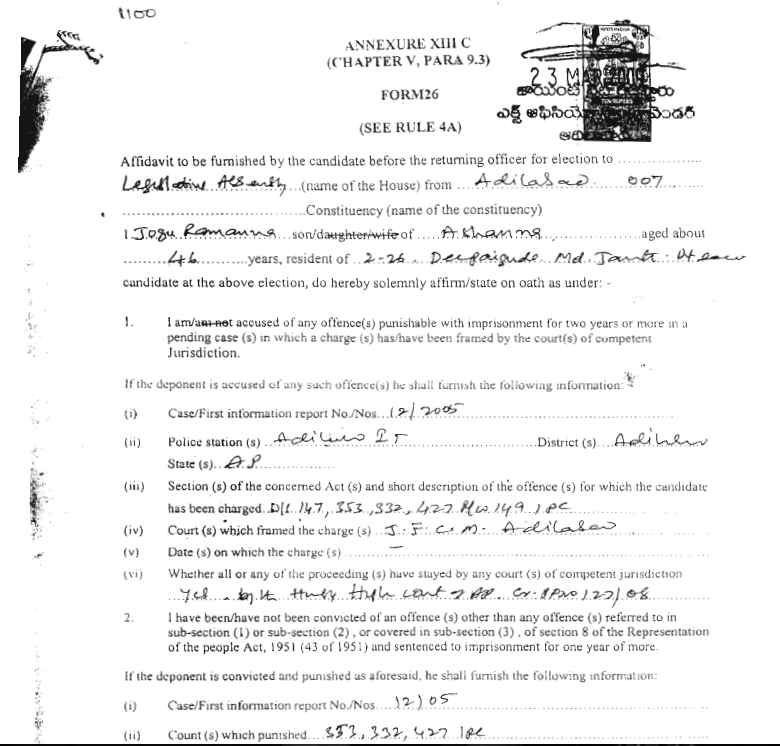
\includegraphics[scale=0.6]{\miningpath/img/affidavit.png}
    \label{fig:affidavit}
  \end{center}
\end{figure}  
\begin{adjustwidth}{2cm}{2cm}
  \footnotesize{The figure shows the first page of a sample affidavit downloaded
    from the web site of the Election Commission of India. Section
    1(iii) lists the sections under the Indian Penal Code under which
    this politician has been charged.}
\end{adjustwidth}     


%%Map of deposit locations
\newpage
\begin{figure}[H]\caption{Map of deposit locations and mineral production}
  \begin{center}
    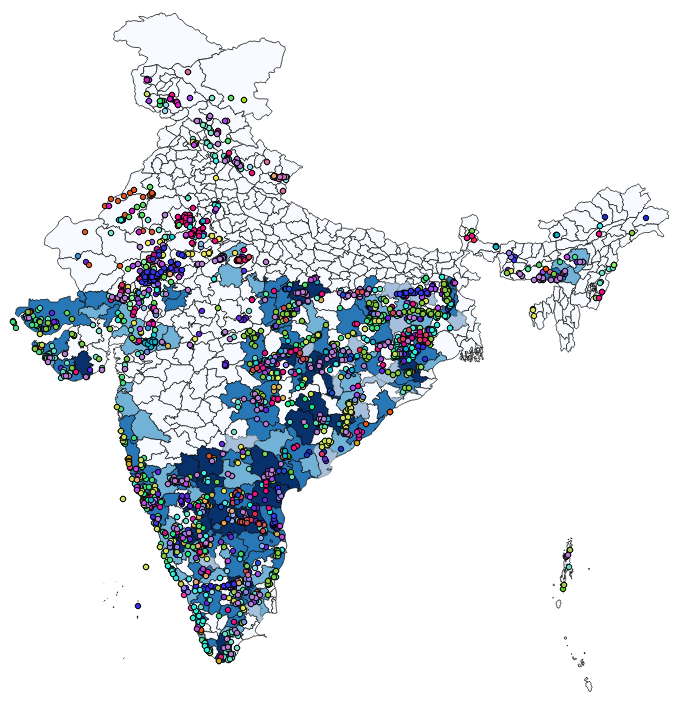
\includegraphics[scale=0.5]{\miningpath/img/mining-prod-map.png}
    \label{fig:deposit_map}
  \end{center}
  \begin{adjustwidth}{2cm}{2cm}
    \footnotesize{Circles indicate the location of mineral deposits,
      color-coded by mineral type. Shaded polygons show districts
      that report mineral production, with darker colors indicating
      higher production deciles. Nearly all states have major mineral
      deposits. The major exceptions are in the Indo-Gangetic Plain
      (Punjab, Uttar Pradesh) and in the northeast. Sources: Mineral
      Atlas of India \cite{GeologicalSurveyofIndia2001} and
      Statistics of Mines in India. }
  \end{adjustwidth}
\end{figure}

%%Price Shock Bar Graph - 2005
\newpage
\begin{figure}[H]\caption{Mineral price shocks 1998-2003}
  \begin{center}
    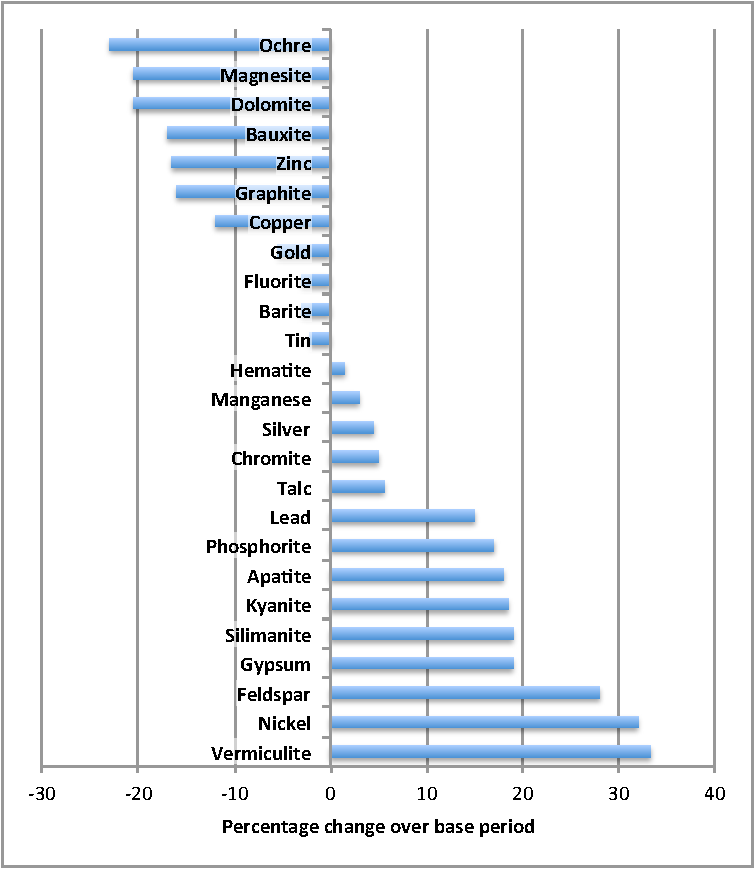
\includegraphics[scale=0.75]{\miningpath/img/mineral_price_chart} 
    \label{fig:bar_pshock_2005}
  \end{center}
  \begin{adjustwidth}{2cm}{2cm}
    \footnotesize{The figure shows mineral-specific price shocks
      calculated from 1998-2003. The price shock is defined as the
      price in 2003 divided by the price in 1998. Source: United
      States Geological Survey.}
  \end{adjustwidth}
\end{figure}

\newpage
\begin{figure}[H]\caption{Map of mineral price shocks (1998-2003)}
  \begin{center}
    \hspace*{-0.9in}
    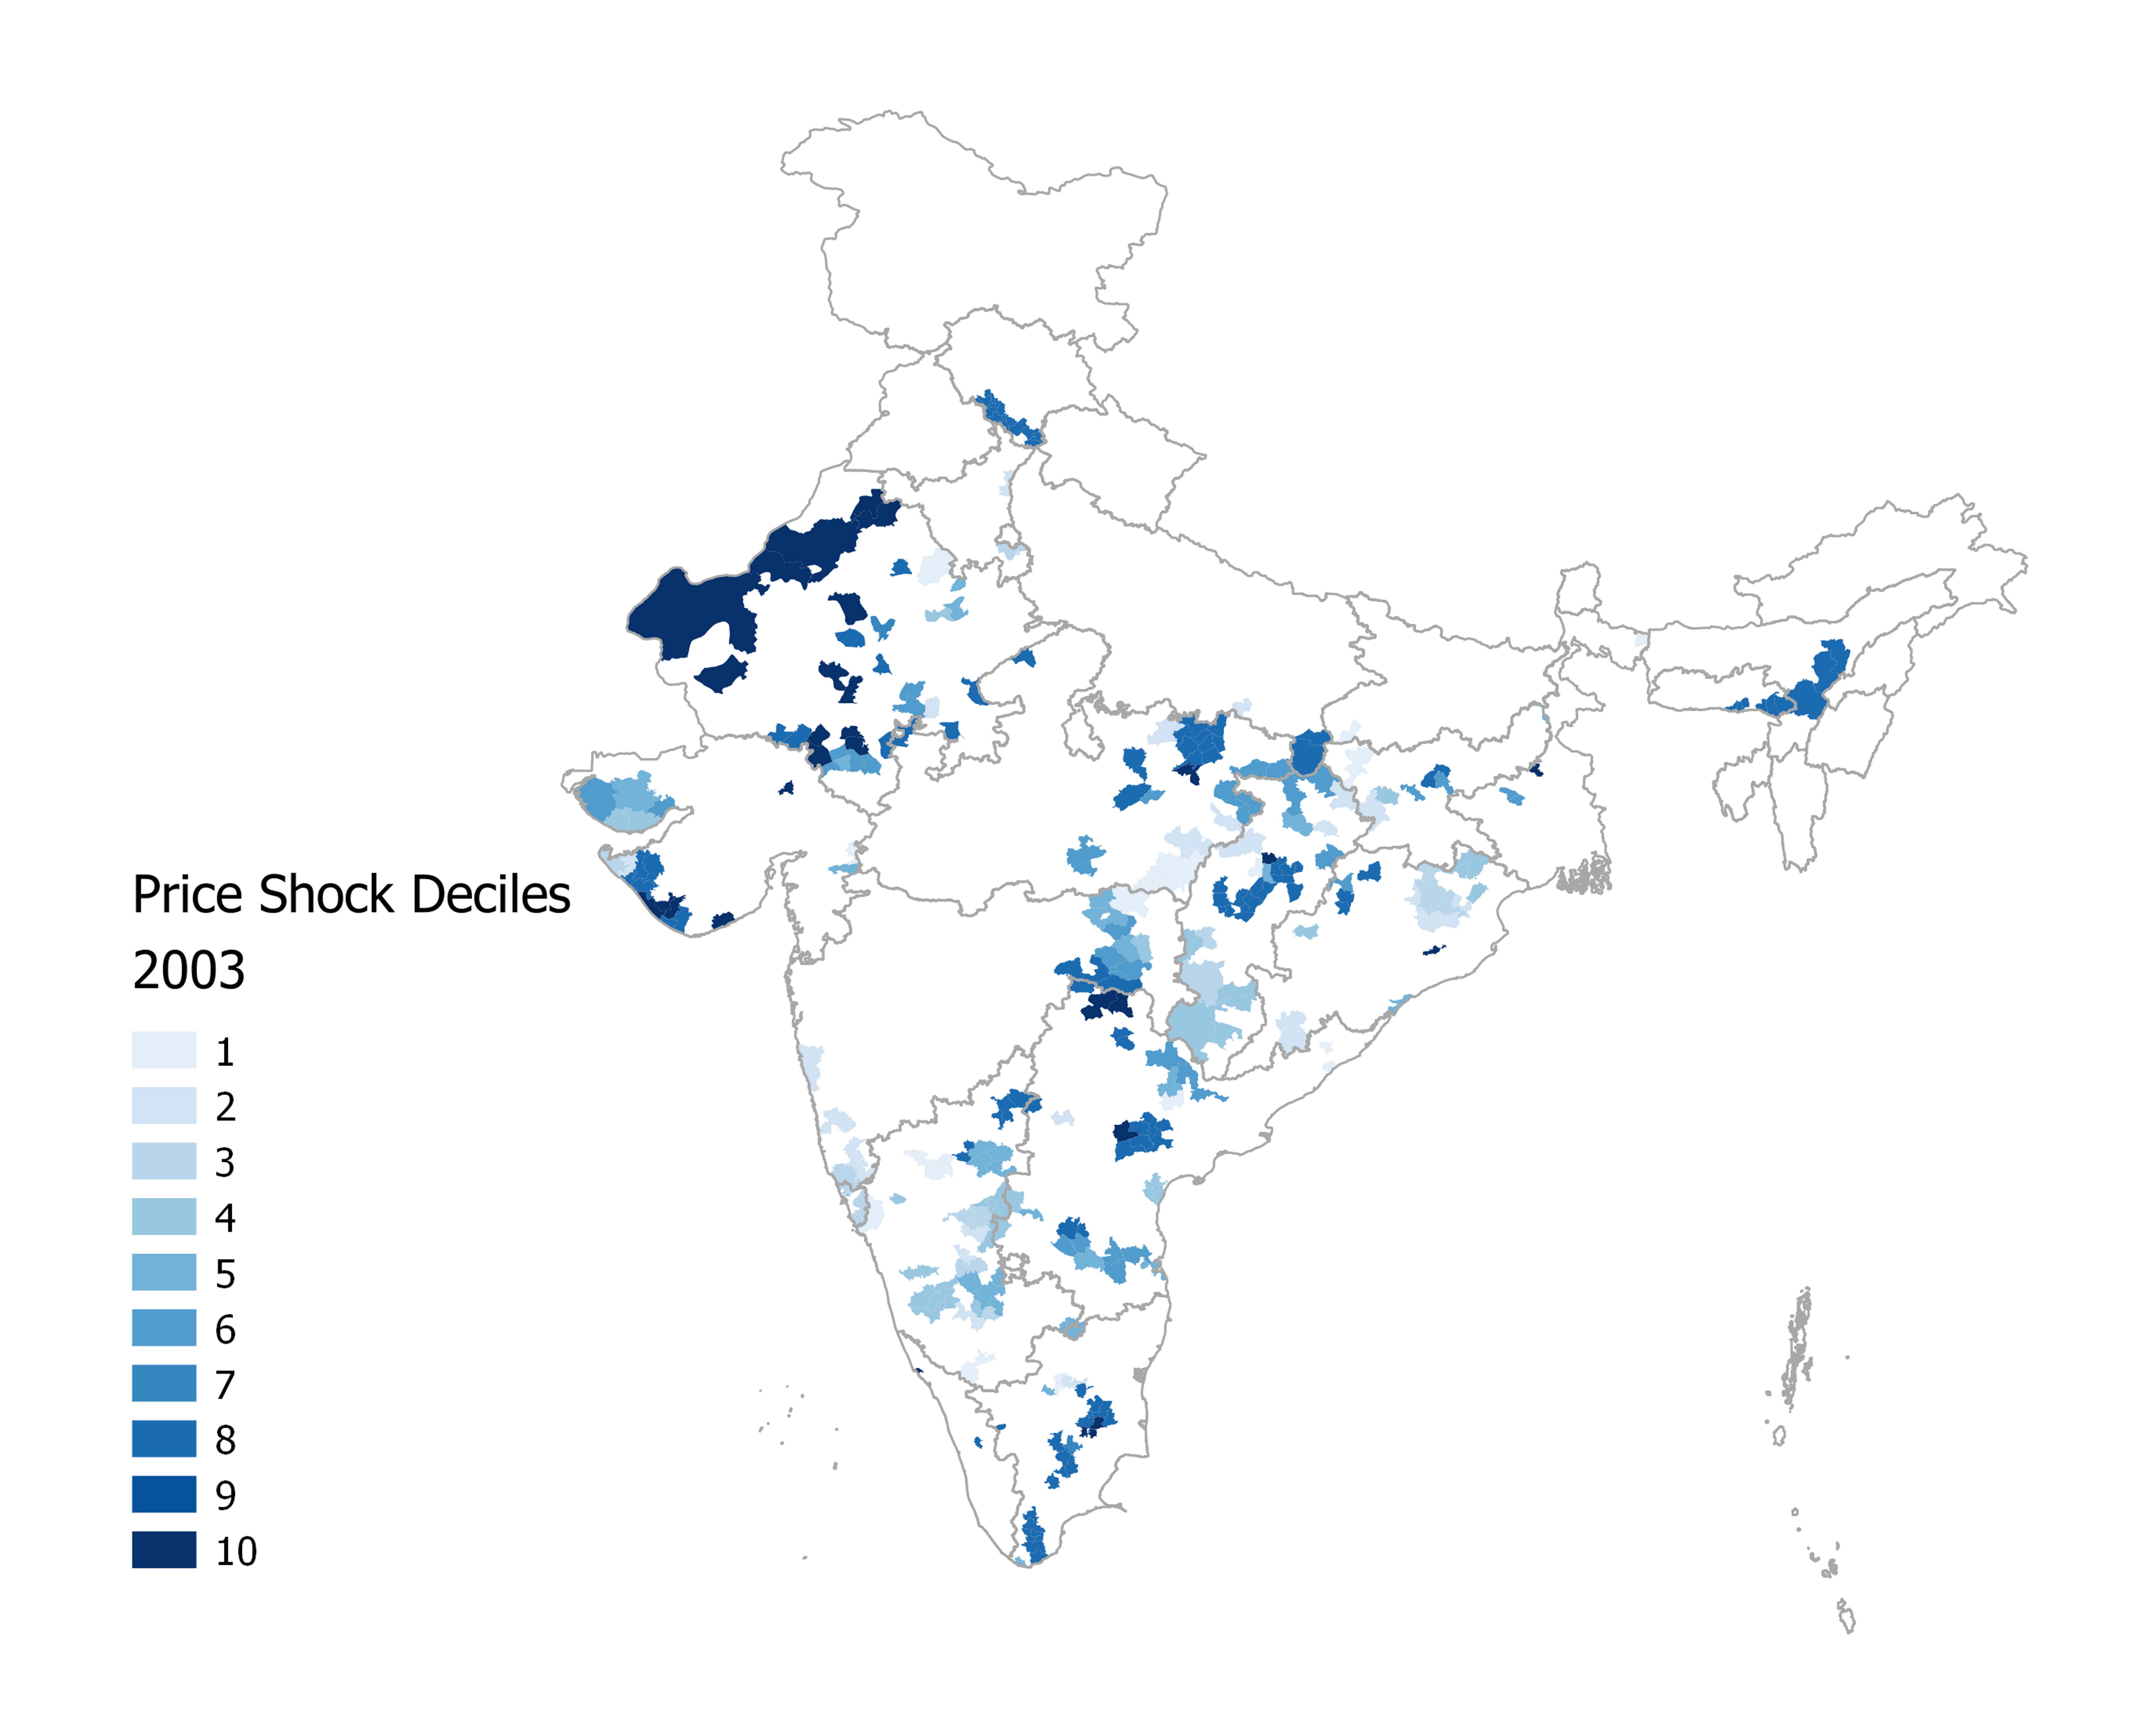
\includegraphics[scale=0.3]{\miningpath/img/mining_heatmap_pshock_deciles_con2007.png} 
    \label{fig:shock_map}
  \end{center}
  \footnotesize{The map shows constituencies (1976-2007
    delimitation) with productive mineral deposits, shaded
    according to the magnitude of the price shock in the period
    1998-2003 (the first shock used in the analysis of crime
    data). Price shocks are defined as the production-weighted
    change in global prices of actively mined minerals in a given
    constituency (see Section~\ref{sec:strat} for more
    information).  The darkest constituencies experienced the
    largest positive price shock.  Unmarked constituencies are
    excluded from our sample because they had no productive mineral
    deposits, or we were not able to match production to a
    deposit. Sources: United States Geological Survey (prices);
    Statistics of Mineral Information, Indian Bureau of Mines
    (production quantities); MLInfoMap (Constituency boundaries).}
\end{figure}

\newpage
\begin{figure}[H]\caption{Histogram of sample price shocks (2003-2017)}
  \begin{center}
    \hspace*{-0.9in}
    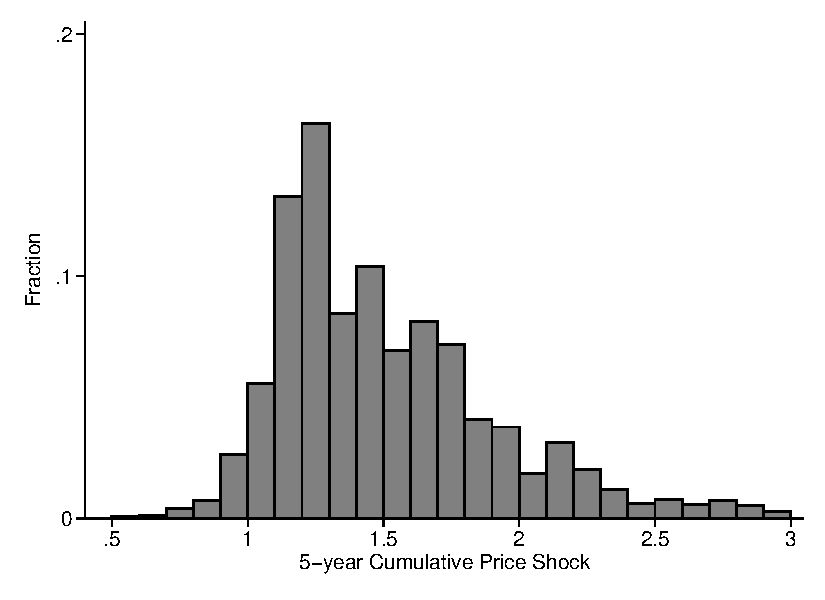
\includegraphics[scale=0.9]{\miningpath/ps5_summary} 
    \label{fig:ps5_hist}
  \end{center}
  \footnotesize{The figure shows the histogram of trailing five-year
    constituency-level price shocks used in the primary analysis
    sample. A price shock is defined as the
    production-value-weighted proportional change in the global
    price of commodities produced in a given constituency from
    period \textit{t=-6} to period \textit{t=-1}, where a given
    election takes place in year \textit{t=0}. See
    Equation~\ref{eq:ps} in Section \ref{sec:strat} for more
    details. The set of election years is 2003 to 2017.}
\end{figure}

  
  %%%%%%%%%%%%%%%%%%%%%%%%%%%%%%%%%
  %% APPENDIX FIGURES AND TABLES %%
  %%%%%%%%%%%%%%%%%%%%%%%%%%%%%%%%%
  \newpage
  \section{Appendix For Online Publication: Additional figures and tables}
  
  % reset appendix counters and prefix with C
  \setcounter{table}{0}
  \renewcommand{\thetable}{A\arabic{table}}
  \setcounter{figure}{0}
  \renewcommand{\thefigure}{A\arabic{figure}}
  \label{app:more_figs}
  %%%%%%%%%%%%%%%%%%%%%%%%%%%%%%%%%
%% DIFFERENT CRIME SUMSTATS %%%%%
%%%%%%%%%%%%%%%%%%%%%%%%%%%%%%%%%
\begin{table}[H]\caption{Criminal Charges Against Politicians
    Contesting Election: \cnewline Summary Statistics}
  \begin{center}
  \begin{tabular}{l c c  c}\hline\hline
\multicolumn{1}{c}{\textbf{Variable}} & \textbf{Mean}
 & \textbf{(Std. Dev.)} & \textbf{N}\\ \hline
Number of open charges listed on affidavit & 1.606 & (5.181)  & 9685\\
Any Charge & 0.32 & (0.466)  & 9685\\
Corruption & 0.103 & (0.304)  & 9563\\
Violent Crime & 0.113 & (0.317)  & 9563\\
Property Crime & 0.075 & (0.263)  & 9563\\
Civil Disorder & 0.134 & (0.341)  & 9563\\
White Collar Crime & 0.028 & (0.166)  & 9563\\
Libel & 0.051 & (0.221)  & 9563\\
\hline\end{tabular}

  \end{center}
  \label{tab:pol_crimes}
  
  \footnotesize{The table shows the distribution of charges faced by
    politicians seeking election in India. The sample period is
    2003--2017. 2003 is the first year that candidates were required
    to file affidavits showing criminal charges.  Corruption is
    defined as theft from a government office, illegally attempting to
    influence a public servant or an election-related crime. Violent
    crime includes actual or attempted assault, armed robbery,
    homicide, kidnapping or sexual assault.}
\end{table}

%%%%%%%%%%%%%%%%%%%%%%%%%%%%%%%%%
%% CON FIXED EFFECT ROBUSTNESS %%
%%%%%%%%%%%%%%%%%%%%%%%%%%%%%%%%%

\begin{table}[H]\caption{Robustness of main results to constituency
    fixed effects}
  \vspace{1cm}
  \small
  \textbf{Panel A: Effect of Price Shocks on Winning Candidate Characteristics}
  \setlength{\linewidth}{.1cm} \begin{center}
\newcommand{\contents}{\begin{tabular}{l*{5}{c}}
\hline\hline
 & BJP & INC & High School & Age & Log Net Assets \\ 
%PYTHON_HEADER
                    &         (1)   &         (2)   &         (3)   &         (4)   &         (5)   \\
\hline
Price shock$_{-6,-1}$&       0.032   &      -0.049   &       0.061*  &      -2.178** &      -0.213   \\
                    &     (0.045)   &     (0.048)   &     (0.036)   &     (1.067)   &     (0.321)   \\
\hline
N                   &        1905   &        1905   &         682   &         710   &         710   \\
r2                  &        0.58   &        0.52   &        0.73   &        0.70   &        0.64   \\
\hline
\multicolumn{6}{p{\linewidth}}{$^{*}p<0.10, ^{**}p<0.05, ^{***}p<0.01$} \\
\multicolumn{6}{p{\linewidth}}{\footnotesize \tablenote}
\end{tabular} }
\setbox0=\hbox{\contents}
\setlength{\linewidth}{\wd0-2\tabcolsep-.25em} \contents \end{center}

  \newline
  \small \textbf{Panel B: Effect of Price Shock on Criminality by Type
    of Crime}
  \setlength{\linewidth}{.1cm} \begin{center}
\newcommand{\contents}{\begin{tabular}{l*{4}{c}}
\hline\hline
 & \underline{Violent} & \underline{Non-violent} & \underline{Corruption} & \underline{Not Corruption} \\ 
%PYTHON_HEADER
                    &         (1)   &         (2)   &         (3)   &         (4)   \\
\hline
Price shock$_{-6,-1}$&       0.135** &      -0.023   &       0.069   &       0.043   \\
                    &     (0.067)   &     (0.069)   &     (0.058)   &     (0.080)   \\
\hline
N                   &         711   &         711   &         711   &         711   \\
r2                  &        0.58   &        0.61   &        0.58   &        0.60   \\
\hline
\multicolumn{5}{p{\linewidth}}{$^{*}p<0.10, ^{**}p<0.05, ^{***}p<0.01$} \\
\multicolumn{5}{p{\linewidth}}{\footnotesize \tablenote}
\end{tabular} }
\setbox0=\hbox{\contents}
\setlength{\linewidth}{\wd0-2\tabcolsep-.25em} \contents \end{center}

  \newline
  \small \textbf{Panel C: Effect of Price Shock on Election Competitiveness}
  \setlength{\linewidth}{.1cm} \begin{center}
\newcommand{\contents}{\begin{tabular}{l*{3}{c}}
\hline\hline
 & \underline{Incumbent} & \underline{Turnout} & \underline{ENOP} \\ 
%PYTHON_HEADER
                    &         (1)   &         (2)   &         (3)   \\
\hline
Price shock$_{-6,-1}$&      -0.021   &       0.005   &       0.155***\\
                    &     (0.053)   &     (0.008)   &     (0.054)   \\
\hline
N                   &        1409   &        1536   &        1414   \\
r2                  &        0.47   &        0.89   &        0.68   \\
\hline
\multicolumn{4}{p{\linewidth}}{$^{*}p<0.10, ^{**}p<0.05, ^{***}p<0.01$} \\
\multicolumn{4}{p{\linewidth}}{\footnotesize \tablenote}
\end{tabular} }
\setbox0=\hbox{\contents}
\setlength{\linewidth}{\wd0-2\tabcolsep-.25em} \contents \end{center}


  \label{tab:con_fe}
  \footnotesize{These three panels shows the robustness of Tables
    \ref{tab:ed_age}, \ref{tab:winner_violence}, and \ref{tab:eci} in
    the body of the paper to the inclusion of constituency fixed
    effects. All rows and columns are identical to those tables in the
    body of the paper, but include constituency fixed effects.} \small
\end{table}

%%%%%%%%%%%%%%%%%%%%%%%%%%%%%%%%
%% Mean Candidate Criminality %%
%%%%%%%%%%%%%%%%%%%%%%%%%%%%%%%%
\begin{table}[H]\caption{Effect of mineral price shocks on non-winner criminality}
  \newcommand{\tablenote}{The table estimates the impact of a local
    mineral price shock on the criminality of candidates who contested
    election but did not win. Criminality is a candidate-level
    indicator that takes the value one if the candidate is facing
    criminal charges. The dependent variable in Columns 1--3 is the
    mean of this indicator across all candidates contesting election
    in each constituency-year. The dependent variable in Columns 4--6
    is the criminality of the second-place candidate in each
    constituency-year.  The price shock is the change in global mineral prices, weighted by
constituency pre-sample production values of each mineral, calculated
over the five years preceding the given election.%
 Columns 1 and 4 estimate
    Equation~\ref{eq:main} on the full sample with state*year fixed
    effects. Columns 2 and 5 add district fixed effects and Columns 3
    and 6 add constituency fixed effects.  All regressions include state-year fixed effects and constituency
controls for the number of deposits within 10km of a constituency, a
constituency-level mineral dispersion index, and baseline (2001)
values of log constituency population, share of the population living
in rural areas, share of villages with electricity and the per
capita number of primary schools.  Standard errors are robust and
clustered at the district level.%
}
  \small \setlength{\linewidth}{.1cm} \begin{center}
\newcommand{\contents}{\begin{tabular}{l*{6}{c}}
\hline\hline
                    &         (1)   &         (2)   &         (3)   &         (4)   &         (5)   &         (6)   \\
\hline
Price shock$_{-6,-1}$&       0.010   &       0.007   &      -0.002   &       0.005   &      -0.015   &      -0.035   \\
                    &     (0.015)   &     (0.017)   &     (0.022)   &     (0.041)   &     (0.045)   &     (0.070)   \\
\hline State-Year F.E.     & Yes & Yes & Yes & Yes & Yes & Yes  \\ 
 District F.E.       & No  & Yes & No  & No  & Yes & No   \\ 
 Constituency F.E.   & No  & No  & Yes & No  & No  & Yes  \\ 
\hline 
Mean Dep. Var. & 0.19 & 0.19 & 0.18 & 0.28 & 0.28 & 0.30 \\ 
%PYTHON_FOOTER
\hline
N                   &         987   &         985   &         807   &         855   &         848   &         631   \\
r2                  &        0.22   &        0.39   &        0.66   &        0.18   &        0.34   &        0.63   \\
\hline
\multicolumn{7}{p{\linewidth}}{$^{*}p<0.10, ^{**}p<0.05, ^{***}p<0.01$} \\
\multicolumn{7}{p{\linewidth}}{\footnotesize \tablenote}
\end{tabular} }
\setbox0=\hbox{\contents}
\setlength{\linewidth}{\wd0-2\tabcolsep-.25em} \contents \end{center}

  \label{tab:app_mean_crim}
\end{table}

%%%%%%%%%%%%%%%%%%%%%%%%%
%% LAGGED PRICE SHOCKS %%
%%%%%%%%%%%%%%%%%%%%%%%%%

\newpage
\begin{table}[H]\caption{Effect of mineral price shocks on candidate asset
    growth and criminal activity \cnewline Robustness to lagged
    price shocks}
  \label{tab:app_ts_lag}
  \newcommand{\tablenote}{The table shows estimates of the impact
    of mineral wealth shocks on asset growth of elected leaders
    and on new criminal charges against them. Results are analogous
    to those in Table~\ref{tab:ts}, but with the inclusion of lagged
    price shocks.  The dependent variable in columns 1--2 is the change in a
    candidate's log net assets over a single electoral term. The price
    shock is the unanticipated change in mineral wealth in that
    electoral term, defined as the change in the global prices of the
    basket of mineral in each constituency, measured from the first
    year after the politician is elected to the end of the electoral
    term. Column 1 estimates the regression on elected officials
    only. In Column 2, the sample includes winners and runners up from
    the first election, and the price shock is interacted with a
    dummy variable indicating the election winner. Columns 3 and 4 run specifications comparable to
    Columns 1 and 2, where the dependent variable is an indicator for
    whether the politician is facing more criminal charges at the end
    of the electoral term than at the beginning. All regressions include state-year fixed effects and constituency
controls for the number of deposits within 10km of a constituency, a
constituency-level mineral dispersion index, and baseline (2001)
values of log constituency population, share of the population living
in rural areas, share of villages with electricity and the per
capita number of primary schools.  Standard errors are robust and
clustered at the district level.%
}
  \setlength{\linewidth}{.1cm} \begin{center}
\newcommand{\contents}{\begin{tabular}{l*{4}{c}}
\hline\hline
 & \multicolumn{2}{c}{\underline{Change in Assets}} & \multicolumn{2}{|c}{\underline{Change in Crime}} \\ 
%PYTHON_HEADER
                    &         (1)   &         (2)   &         (3)   &         (4)   \\
\hline
Price shock$_{+1,+5}$&       0.267***&      -0.045   &       0.216***&      -0.045   \\
                    &     (0.101)   &     (0.165)   &     (0.062)   &     (0.087)   \\
Price shock$_{+1,+5}$ * Winner&               &       0.302*  &               &       0.244** \\
                    &               &     (0.168)   &               &     (0.100)   \\
Winner              &               &      -0.142   &               &      -0.420** \\
                    &               &     (0.297)   &               &     (0.201)   \\
Price shock$_{-5,-1}$ (lagged)&       0.095   &       0.191** &       0.023   &      -0.010   \\
                    &     (0.103)   &     (0.092)   &     (0.058)   &     (0.070)   \\
Price shock$_{-5,-1}$ (lagged) * Winner&               &      -0.073   &               &       0.021   \\
                    &               &     (0.119)   &               &     (0.081)   \\
\hline
State-Year F.E. & Yes & Yes & Yes & Yes \\ 
\hline 
Mean Dep. Var. & 1.02 & 0.98 & 0.18 & 0.20 \\ 
%PYTHON_FOOTER
\hline
N                   &         448   &         696   &         364   &         629   \\
r2                  &        0.40   &        0.33   &        0.23   &        0.18   \\
\hline
\multicolumn{5}{p{\linewidth}}{$^{*}p<0.10, ^{**}p<0.05, ^{***}p<0.01$} \\
\multicolumn{5}{p{\linewidth}}{\footnotesize \tablenote}
\end{tabular} }
\setbox0=\hbox{\contents}
\setlength{\linewidth}{\wd0-2\tabcolsep-.25em} \contents \end{center}

\end{table}

\newpage
%%%%%%%%%%%%%%%%%%%%%%%%%%%%%%%%%%%%%%%
%% EMPLOYMENT GROWTH / BARTIK SHOCKS %%
%%%%%%%%%%%%%%%%%%%%%%%%%%%%%%%%%%%%%%%
\begin{table}[H]\caption{Effect of employment shocks on candidate
    selection and behavior}
  \vspace{1cm}
  \small
  \textbf{Panel A: Constituency-Level Non-Farm Employment Growth}
  \footnotesize \setlength{\linewidth}{.1cm} \begin{center}
\newcommand{\contents}{\begin{tabular}{l*{5}{c}}
\hline\hline
 & \underline{Crim Winner} & \multicolumn{2}{c}{\underline{Change in Assets}} & \multicolumn{2}{c}{\underline{Change in Crime}} \\ 
%PYTHON_HEADER
                    &         (1)   &         (2)   &         (3)   &         (4)   &         (5)   \\
\hline
Pre-Election Growth &      -0.003   &               &               &               &               \\
                    &     (0.016)   &               &               &               &               \\
Growth in Electoral Term&               &       0.108   &       0.077   &      -0.045   &       0.224***\\
                    &               &     (0.211)   &     (0.136)   &     (0.046)   &     (0.071)   \\
Winner              &               &               &       0.190   &               &       0.031   \\
                    &               &               &     (0.128)   &               &     (0.056)   \\
Winner * Growth in Electoral Term&               &               &       0.029   &               &      -0.245***\\
                    &               &               &     (0.207)   &               &     (0.072)   \\
Constant            &       0.339***&       1.178***&       1.011***&       0.224***&       0.198***\\
                    &     (0.009)   &     (0.085)   &     (0.104)   &     (0.030)   &     (0.047)   \\
\hline
State-Year F.E. & Yes & Yes & Yes & Yes & Yes \\ 
\hline 
Mean Dep. Var. & 0.34 & 1.21 & 1.17 & 0.21 & 0.25  \\ 
%PYTHON_FOOTER
\hline
N                   &        4427   &         213   &         335   &         219   &         349   \\
r2                  &        0.10   &        0.12   &        0.09   &        0.13   &        0.14   \\
\hline
\multicolumn{6}{p{\linewidth}}{$^{*}p<0.10, ^{**}p<0.05, ^{***}p<0.01$} \\
\multicolumn{6}{p{\linewidth}}{\footnotesize \tablenote}
\end{tabular} }
\setbox0=\hbox{\contents}
\setlength{\linewidth}{\wd0-2\tabcolsep-.25em} \contents \end{center}
 \newline

  \newcommand{\tablenote}{The table replicates the main results of the
    paper using shocks to non-farm sector employment instead of
    mineral wealth shocks. The independent variable in Panel A is
    constituency-level non-farm employment growth; in Panel B, it is
    \textit{predicted} non-farm employment growth from a Bartik
    specification. Column 1 shows a regression of a criminal winner
    indicator on employment growth in the period before the
    election. Columns 2 and 3 show regressions of the change in
    candidate assets on employment growth during the candidate's term
    in office. Columns 4 and 5 show regressions of an indicator that
    takes the value one if a candidate has accumulated additional
    criminal charges during the electoral term, on employment growth
    during the candidate's term in office. Columns 2 and 4 are
    restricted to sitting MLAs (i.e. election winners) only; Columns 3
    and 5 include runners-up in the last election as a control
    group. All regressions include state-year fixed effects and the
    standard set of constituency controls. Standard errors are robust
    and clustered at the district level.}
  \small \textbf{Panel B: Bartik-Predicted Constituency-Level Non-Farm Employment Growth}
  \footnotesize \setlength{\linewidth}{.1cm} \begin{center}
\newcommand{\contents}{\begin{tabular}{l*{5}{c}}
\hline\hline
 & \underline{Crim Winner} & \multicolumn{2}{c}{\underline{Change in Assets}} & \multicolumn{2}{c}{\underline{Change in Crime}} \\ 
%PYTHON_HEADER
                    &         (1)   &         (2)   &         (3)   &         (4)   &         (5)   \\
\hline
Bartik Predicted Pre-Election Growth&       0.078   &               &               &               &               \\
                    &     (0.103)   &               &               &               &               \\
Predicted Growth in Electoral Term&               &      -1.309   &      -2.442   &      -0.287   &       0.142   \\
                    &               &     (0.950)   &     (1.584)   &     (0.316)   &     (0.668)   \\
Winner              &               &               &      -0.289   &               &       0.068   \\
                    &               &               &     (0.714)   &               &     (0.301)   \\
Winner * Predicted Growth in Electoral Term&               &               &       1.158   &               &      -0.313   \\
                    &               &               &     (1.694)   &               &     (0.700)   \\
Constant            &       0.308***&       1.757***&       2.056***&       0.329** &       0.227   \\
                    &     (0.039)   &     (0.397)   &     (0.656)   &     (0.138)   &     (0.281)   \\
\hline
State-Year F.E. & Yes & Yes & Yes & Yes & Yes \\ 
\hline 
Mean Dep. Var. & 0.34 & 1.21 & 1.17 & 0.21 & 0.25 \\ 
%PYTHON_FOOTER
\hline
N                   &        4427   &         213   &         335   &         219   &         349   \\
r2                  &        0.10   &        0.13   &        0.10   &        0.13   &        0.12   \\
\hline
\multicolumn{6}{p{\linewidth}}{$^{*}p<0.10, ^{**}p<0.05, ^{***}p<0.01$} \\
\multicolumn{6}{p{\linewidth}}{\footnotesize \tablenote}
\end{tabular} }
\setbox0=\hbox{\contents}
\setlength{\linewidth}{\wd0-2\tabcolsep-.25em} \contents \end{center}

  \label{tab:app_ec_growth_bartik}
\end{table}

\newpage
%%%%%%%%%%%%%%%%%%%%%%%%%%%%%%%%%%%%%
%% RAINFALL SHOCKS ON ALL OUTCOMES %%
%%%%%%%%%%%%%%%%%%%%%%%%%%%%%%%%%%%%%
\begin{table}[H]\caption{Effect of rainfall shocks on candidate
    selection and behavior}
  \newcommand{\tablenote}{The table replicates the main results of the
    paper using precipitation shocks instead of mineral wealth shocks.
    Column 1 shows a regression of a criminal winner indicator on
    rainfall in the year before the election. Column 2 uses average
    rainfall in the five years before the election.  Columns 3 and 4
    show regressions of the change in candidate assets on average
    rainfall during the candidate's term in office. Columns 5 and 6
    show regressions of an indicator that takes the value one if a
    candidate has accumulated additional criminal charges during the
    electoral term, on average rainfall during the candidate's term in
    office. Columns 3 and 5 are restricted to sitting MLAs
    (i.e. election winners) only; Columns 4 and 6 include runners-up
    in the last election as a control group.  Rainfall in each year is
    measured as total rainfall in the month of monsoon arrival.  All
    regressions include state-year fixed effects and the standard set
    of constituency controls. Standard errors are robust and clustered
    at the district level.
  }  \small
  \setlength{\linewidth}{.1cm} \begin{center}
\newcommand{\contents}{\begin{tabular}{l*{6}{c}}
\hline\hline
 & \multicolumn{2}{c}{\underline{Criminal Winner}} & \multicolumn{2}{c}{\underline{Change in Assets}} & \multicolumn{2}{c}{\underline{Change in Crime}} \\ 
%PYTHON_HEADER
                    &         (1)   &         (2)   &         (3)   &         (4)   &         (5)   &         (6)   \\
\hline
Precip. Year Before Election&       0.001   &               &               &               &               &               \\
                    &     (0.009)   &               &               &               &               &               \\
Precip. 5 Years Before Election&               &      -0.017   &               &               &               &               \\
                    &               &     (0.019)   &               &               &               &               \\
Precip. During Electoral Term&               &               &       0.159   &       0.190   &      -0.014   &       0.108   \\
                    &               &               &     (0.223)   &     (0.205)   &     (0.099)   &     (0.109)   \\
Winner              &               &               &               &       0.194** &               &      -0.052   \\
                    &               &               &               &     (0.084)   &               &     (0.041)   \\
Precip. During Term * Winner&               &               &               &       0.150   &               &      -0.023   \\
                    &               &               &               &     (0.161)   &               &     (0.081)   \\
Constant            &       0.306***&       0.307***&       1.098***&       0.949***&       0.181***&       0.247***\\
                    &     (0.006)   &     (0.005)   &     (0.058)   &     (0.064)   &     (0.026)   &     (0.036)   \\
\hline
State-Year F.E. & Yes & Yes & Yes & Yes & Yes & Yes \\ 
\hline 
Mean Dep. Var. & 0.31 & 0.31 & 1.08 & 1.03 & 0.18 & 0.20 \\ 
%PYTHON_FOOTER
\hline
N                   &        9274   &        9274   &         356   &         596   &         361   &         612   \\
r2                  &        0.13   &        0.13   &        0.19   &        0.15   &        0.17   &        0.13   \\
\hline
\multicolumn{7}{p{\linewidth}}{$^{*}p<0.10, ^{**}p<0.05, ^{***}p<0.01$} \\
\multicolumn{7}{p{\linewidth}}{\footnotesize \tablenote}
\end{tabular} }
\setbox0=\hbox{\contents}
\setlength{\linewidth}{\wd0-2\tabcolsep-.25em} \contents \end{center}

  \label{tab:app_precip}
\end{table}

%%%%%%%%%%%%%%%%%%%%%%%
%% ROBUSTNESS TABLES %%
%%%%%%%%%%%%%%%%%%%%%%%
\newpage
\begin{table}[H]\caption{Effect of mineral price shocks on winning candidate
    criminality \cnewline
    Alternate deposit definitions}
  \label{tab:app_deps_only}
  \newcommand{\tablenote}{ This table estimates the impact of a
    local mineral price shock on the criminality of the local
    elected leader, with specifications parallel to those in Table
    \ref{tab:winner_crim}. The price shock variable is a weighted
    sum of global price shocks to the minerals present in a
    constituency. The dependent variable is an indicator that takes
    the value one if the local election winner is facing criminal
    charges.  Columns 1 through 3 define price shocks using mineral
    deposits strictly within constituency boundaries, under
    different fixed effect specifications. In contrast,
    Table~\ref{tab:winner_crim} weights price shocks using
    proximity to deposits that are close to constituencies.
    Columns 4 through 6 weight price shocks with the number of
    mineral deposits in a constituency, irrespective of whether
    production is reported in that constituency, under different
    fixed effect specifications. In contrast,
    Table~\ref{tab:winner_crim} uses pre-sample mineral output
    values as weights.  Sample size is lower than Table
    \ref{tab:winner_crim} as some constituencies are close to
    deposits but do not contain deposits. All regressions include state-year fixed effects and constituency
controls for the number of deposits within 10km of a constituency, a
constituency-level mineral dispersion index, and baseline (2001)
values of log constituency population, share of the population living
in rural areas, share of villages with electricity and the per
capita number of primary schools.  Standard errors are robust and
clustered at the district level.%
}
  \setlength{\linewidth}{.1cm} \begin{center}
\newcommand{\contents}{\begin{tabular}{l*{6}{c}}
\hline\hline
 & \multicolumn{3}{c}{\underline{Exact Deposit Locations}} & \multicolumn{3}{c}{\underline{Deposits Only}} \\ 
%PYTHON_HEADER
                    &         (1)   &         (2)   &         (3)   &         (4)   &         (5)   &         (6)   \\
\hline
Price shock$_{-6,-1}$&       0.131***&       0.107** &       0.118** &       0.040** &       0.038** &       0.051*  \\
                    &     (0.039)   &     (0.041)   &     (0.056)   &     (0.016)   &     (0.016)   &     (0.028)   \\
\hline State-Year F.E. & Yes & Yes & Yes & Yes & Yes & Yes \\ 
District   F.E.     & No  & Yes & No & No  & Yes & No \\ 
Constituency   F.E. & No  & No  & Yes & No  & No  & Yes \\ 
\hline 
Mean Dep. Var. & 0.33 & 0.33 & 0.32 & 0.30 & 0.30 & 0.30 \\ 
%PYTHON_FOOTER
\hline
N                   &         628   &         625   &         484   &        3280   &        3270   &        1905   \\
r2                  &        0.18   &        0.39   &        0.69   &        0.13   &        0.25   &        0.66   \\
\hline
\multicolumn{7}{p{\linewidth}}{$^{*}p<0.10, ^{**}p<0.05, ^{***}p<0.01$} \\
\multicolumn{7}{p{\linewidth}}{\footnotesize \tablenote}
\end{tabular} }
\setbox0=\hbox{\contents}
\setlength{\linewidth}{\wd0-2\tabcolsep-.25em} \contents \end{center}

\end{table}

\newpage
\begin{landscape}
  \begin{table}[H]\caption{Effect of price shocks on winning candidate
      criminality \cnewline Alternate price shock definitions}
    \label{tab:app_alt_pshock_regs}
    \newcommand{\tablenote}{ This table estimates the impact of a
      local mineral price shock on the criminality of the local
      elected leader, under alternate price shock
      definitions. The price shock is the change in global mineral prices, weighted by
constituency pre-sample production values of each mineral, calculated
over the five years preceding the given election.%
 The dependent variable is an
      indicator that takes the value one if the local election winner
      is facing criminal charges. Column 1 weights mineral deposits
      based on baseline district-level mineral output measured from 1990--2003,
      instead of 1990--2013. Column 2 defines the price shock from 5
      years before the election date to the present date (as opposed
      to Table \ref{tab:winner_crim} which uses 6 years before to 1
      year before). Column 3, 4 and 5 define mineral constituencies as
      those with production of at least (3) \$1 in any one year;
      \$50,000 in one year; or (5) \$200,000 in any year. In
      Table~\ref{tab:winner_crim}, the threshold is \$100,000. Column
      6 presents the main specification from
      Table~\ref{tab:winner_crim}, with standard errors clustered at
      the state level. Column 7 shows estimates from a placebo
      specification, where the treatment variable is the change in
      value of mineral deposits in constituencies that report zero
      production, i.e. constituencies with unproductive mineral
      deposits. All regressions include state-year fixed effects and constituency
controls for the number of deposits within 10km of a constituency, a
constituency-level mineral dispersion index, and baseline (2001)
values of log constituency population, share of the population living
in rural areas, share of villages with electricity and the per
capita number of primary schools.  Standard errors are robust and
clustered at the district level.%
 }
    \setlength{\linewidth}{.1cm} \begin{center}
\newcommand{\contents}{\begin{tabular}{l*{7}{c}}
\hline\hline
 & Baseline   & Shock_{-5,0} & Prod above & Prod above & Prod above & State    & Placebo \\ &  1990-2003 &              &  0   &   USD 50k   &  USD 200k  & Clusters & Fixed Effects &  \\ 
%PYTHON_HEADER
                    &         (1)   &         (2)   &         (3)   &         (4)   &         (5)   &         (6)   &         (7)   \\
\hline
Price Shock         &       0.136***&       0.134** &       0.087***&       0.086** &       0.120** &       0.097** &       0.029   \\
                    &     (0.046)   &     (0.054)   &     (0.032)   &     (0.041)   &     (0.048)   &     (0.037)   &     (0.043)   \\
\hline State-Year F.E.      & Yes & Yes & Yes & Yes & Yes & Yes & Yes \\ 
       District-Year F.E.   & Yes & Yes & Yes & Yes & Yes & Yes & Yes \\ 
\hline 
Mean Dep. Var. & 0.35 & 0.33 & 0.32 & 0.34 & 0.34 & 0.33 & 0.25 \\ 
%PYTHON_FOOTER
\hline
N                   &         720   &         948   &        1726   &        1063   &         780   &         946   &         679   \\
r2                  &        0.34   &        0.34   &        0.26   &        0.33   &        0.36   &        0.35   &        0.44   \\
\hline
\multicolumn{8}{p{\linewidth}}{$^{*}p<0.10, ^{**}p<0.05, ^{***}p<0.01$} \\
\multicolumn{8}{p{\linewidth}}{\footnotesize \tablenote}
\end{tabular} }
\setbox0=\hbox{\contents}
\setlength{\linewidth}{\wd0-2\tabcolsep-.25em} \contents \end{center}

  \end{table}
\end{landscape}

\newpage
\begin{landscape}
  \begin{table}[H]\caption{Effect of mineral price shocks on candidate asset
      growth and criminal activity \cnewline Alternate
      price shock definitions}
    \label{tab:app_ts_robust}
    \newcommand{\tablenote}{ The table shows estimates of the impact
      of mineral wealth shocks on asset growth of elected leaders,
      and on new criminal charges against them. Results are analogous
      to those in Table~\ref{tab:ts}, but with alternate definitions
      of price shocks.  The dependent variable in columns 1, 3, 5 and
      7 is the change in a candidate's log net assets over a single
      electoral term. The dependent variable in columns 2, 4, 6 and 8
      is an indicator for whether the politician is facing more
      criminal charges at the end of the electoral term than at the
      beginning The price shock is the unanticipated change in
      mineral wealth in that electoral term, defined as the change in
      the global prices of the basket of mineral in each
      constituency, measured from the first year after the politician
      is elected to the end of the electoral term.  Columns 1 and 2
      show results based strictly on mineral deposits, ignoring
      production data. Columns 3 and 4 define production using all
      years of data. Columns 5 and 6 define mineral constituencies at
      the lower production threshold, and Columns 7 and 8 do so at
      the higher production threshold.  All regressions include state-year fixed effects, district fixed
effects and constituency controls for the number of deposits within
10km of a constituency, a constituency-level mineral dispersion index,
and baseline (2001) values of log constituency population, share of
the population living in rural areas, share of villages with
electricity and the per capita number of primary schools.  Standard
errors are robust and clustered at the district level.%
 }
    \setlength{\linewidth}{.1cm} \begin{center}
\newcommand{\contents}{\begin{tabular}{l*{8}{c}}
\hline\hline
 & Assets & Crime & Assets & Crime & Assets & Crime & Assets & Crime \\ 
%PYTHON_HEADER
                    &         (1)   &         (2)   &         (3)   &         (4)   &         (5)   &         (6)   &         (7)   &         (8)   \\
\hline
Price shock$_{+1,+5}$&       0.279***&       0.190** &       0.331***&       0.141** &       0.256** &       0.220***&       0.222** &       0.212***\\
                    &     (0.105)   &     (0.078)   &     (0.118)   &     (0.067)   &     (0.117)   &     (0.070)   &     (0.100)   &     (0.063)   \\
\hline
State-Year F.E. & Yes & Yes & Yes & Yes & Yes & Yes & Yes & Yes \\ 
\hline 
N                   &         301   &         248   &         291   &         240   &         362   &         290   &         477   &         370   \\
r2                  &        0.43   &        0.29   &        0.43   &        0.24   &        0.41   &        0.24   &        0.37   &        0.24   \\
\hline
\multicolumn{9}{p{\linewidth}}{$^{*}p<0.10, ^{**}p<0.05, ^{***}p<0.01$} \\
\multicolumn{9}{p{\linewidth}}{\footnotesize \tablenote}
\end{tabular} }
\setbox0=\hbox{\contents}
\setlength{\linewidth}{\wd0-2\tabcolsep-.25em} \contents \end{center}

  \end{table}
\end{landscape}

%%%%%%%%%%%%%%%%%%%%%%%%
%% SPATIAL SPILLOVERS %%
%%%%%%%%%%%%%%%%%%%%%%%%
\newpage
\begin{table}[H]\caption{Effect of mineral price shocks on winning
    candidate criminality \cnewline Spatial Spillovers}
  \newcommand{\tablenote}{The table estimates the impact of local
    mineral price shocks on the criminality elected politicians in
    neighboring constituencies.  The dependent variable is the share
    of neighboring constituencies in which the election winner faces
    criminal charges.  The price shock is the average price shock in
    the neighboring constituencies. The row marked ``Price Shock to
    Neighbors'' is the price shock in the reference constituency.  In
    both cases, the price shock is a change in global mineral prices,
    weighted by constituency pre-sample production values of each
    mineral, calculated over the five years preceding the given
    election.  Column 1 estimates Equation~\ref{eq:main} on the full
    sample with state*year fixed effects, with the additional
    neighboring price shock variable. Columns 2 and 3 respectively add
    district and constituency fixed effects. Column 4 shows the marginal effect from a probit
    estimation of a similar specification to that in Column
    1. All regressions include state-year fixed effects and constituency
controls for the number of deposits within 10km of a constituency, a
constituency-level mineral dispersion index, and baseline (2001)
values of log constituency population, share of the population living
in rural areas, share of villages with electricity and the per
capita number of primary schools.  Standard errors are robust and
clustered at the district level.%
 }  \small
  \setlength{\linewidth}{.1cm} \begin{center}
\newcommand{\contents}{\begin{tabular}{l*{4}{c}}
\hline\hline
                    &         (1)   &         (2)   &         (3)   &         (4)   \\
\hline
Price Shock         &       0.163***&       0.194***&       0.202***&       0.118*  \\
                    &     (0.053)   &     (0.059)   &     (0.071)   &     (0.070)   \\
Price Shock to Neighbors&      -0.044   &      -0.052   &      -0.050   &      -0.035   \\
                    &     (0.045)   &     (0.044)   &     (0.051)   &     (0.058)   \\
\hline State-Year F.E.      & Yes & Yes & Yes & Yes \\ 
 District F.E.        & No  & Yes & Yes & No  \\ 
 Constituency F.E.    & No  & No  & Yes & No  \\ 
\hline 
Mean Dep. Var. & 0.33 & 0.33 & 0.33 & 0.33 \\ 
%PYTHON_FOOTER
\hline
N                   &         865   &         862   &         650   &         786   \\
r2                  &        0.37   &        0.57   &        0.75   &               \\
\hline
\multicolumn{5}{p{\linewidth}}{$^{*}p<0.10, ^{**}p<0.05, ^{***}p<0.01$} \\
\multicolumn{5}{p{\linewidth}}{\footnotesize \tablenote}
\end{tabular} }
\setbox0=\hbox{\contents}
\setlength{\linewidth}{\wd0-2\tabcolsep-.25em} \contents \end{center}

  \label{tab:app_spill}
\end{table}

%%%%%%%%%%%%%%%%%%%%%%%%%%%%%%%%%%%%%%%%%%%%
%% ALTERNATE CONTINUOUS CRIME DEFINITIONS %%
%%%%%%%%%%%%%%%%%%%%%%%%%%%%%%%%%%%%%%%%%%%%
\newpage
\begin{table}[H]\caption{Adverse selection and moral hazard tests \cnewline
    Alternate crime definitions}
  \newcommand{\tablenote}{This table tests the robustness of results
    in Tables~\ref{tab:winner_crim} and \ref{tab:ts} to alternate
    definitions of the criminality of the winner. Columns 1 and 2 estimate the impact of local
    pre-election mineral price shocks on the criminality of the local elected
    politician. The dependent variable in Column 1 is the number of
    criminal charges faced by the winner; in Column 2 it is the log of
    the number of criminal charges plus one. Columns 3 and 4 estimate
    the impact of post-election mineral price shocks on the number of
    charges faced by the elected leader in a constituency. These columns
    again show the effect on the number of charges and the log number of charges.
    All columns include state and year fixed effects. Columns 1 and 2
    include district fixed effects. All regressions include state-year fixed effects and constituency
controls for the number of deposits within 10km of a constituency, a
constituency-level mineral dispersion index, and baseline (2001)
values of log constituency population, share of the population living
in rural areas, share of villages with electricity and the per
capita number of primary schools.  Standard errors are robust and
clustered at the district level.%

  } \small \setlength{\linewidth}{.1cm} \begin{center}
\newcommand{\contents}{\begin{tabular}{l*{4}{c}}
\hline\hline
 & \multicolumn{2}{c}{\underline{Adverse Selection}} & \multicolumn{2}{c}{\underline{Moral Hazard (Differences)}} \\  & Num Crime & Log Num Crime & Num Crime & Log Num Crime  \\ 
%PYTHON_HEADER
                    &         (1)   &         (2)   &         (3)   &         (4)   \\
\hline
Price shock$_{-6,-1}$&       0.646***&       0.201***&               &               \\
                    &     (0.172)   &     (0.055)   &               &               \\
Price shock$_{+1,+5}$&               &               &       1.082** &       0.209** \\
                    &               &               &     (0.517)   &     (0.091)   \\
\hline
State-Year F.E. & Yes & Yes & Yes & Yes \\ 
\hline 
Mean Dep. Var. & 1.33 & 0.43 & -0.55 & -0.05 \\ 
%PYTHON_FOOTER
\hline
N                   &         948   &         948   &         364   &         364   \\
r2                  &        0.20   &        0.22   &        0.56   &        0.55   \\
\hline
\multicolumn{5}{p{\linewidth}}{$^{*}p<0.10, ^{**}p<0.05, ^{***}p<0.01$} \\
\multicolumn{5}{p{\linewidth}}{\footnotesize \tablenote}
\end{tabular} }
\setbox0=\hbox{\contents}
\setlength{\linewidth}{\wd0-2\tabcolsep-.25em} \contents \end{center}

  \label{tab:app_crime_alt}
\end{table}



%%%%%%%%%%%%%%%%%%%%%%%%%
%% IRON/COAL EXCLUSION %%
%%%%%%%%%%%%%%%%%%%%%%%%%
\newpage
\begin{landscape}
  \begin{table}[H]\caption{Effect of price shocks on winning candidate
      criminality \cnewline Iron, coal, conflict exclusions}
    \label{tab:app_no_iron_coal_regs}
    \newcommand{\tablenote}{ This table estimates the impact of a
      local mineral price shock on the criminality of the local elected
      leader, excluding certain effects in coal- and iron-producing
      regions. The price shock is the change in global mineral prices, weighted by
constituency pre-sample production values of each mineral, calculated
over the five years preceding the given election.%
 The dependent variable is an
      indicator that takes the value one if the local election winner
      is facing criminal charges. Column 1 calculates price shocks
      with coal deposits excluded; Column 2 excludes iron deposits
      from the price shock, and Column 3 excludes both. Columns 4-6
      drop constituencies entirely if they have (4) a coal deposit,
      (5) an iron deposit, or (6) either a coal or iron deposit. Column
      7 excludes the four states with the greatest Naxalite presence
      (Orissa, Andhra Pradesh, Jharkhand and Chhattisgarh). Column 8
      excludes districts with at least Naxalite conflict-related death
      between 2005--2010.
      All regressions include state-year fixed effects, district fixed
effects and constituency controls for the number of deposits within
10km of a constituency, a constituency-level mineral dispersion index,
and baseline (2001) values of log constituency population, share of
the population living in rural areas, share of villages with
electricity and the per capita number of primary schools.  Standard
errors are robust and clustered at the district level.%
 } \footnotesize
    \setlength{\linewidth}{.1cm} \begin{center}
\newcommand{\contents}{\begin{tabular}{l*{8}{c}}
\hline\hline
                    &         (1)   &         (2)   &         (3)   &         (4)   &         (5)   &         (6)   &         (7)   &         (8)   \\
\hline
Price shock$_{-6,-1}$&       0.100** &       0.142***&       0.128***&       0.118***&       0.171***&       0.178***&       0.129** &       0.163***\\
                    &     (0.040)   &     (0.043)   &     (0.040)   &     (0.045)   &     (0.054)   &     (0.055)   &     (0.057)   &     (0.047)   \\
\hline Price Shock   & No coal & No iron & No coal/iron & No coal & No iron & No coal/iron & All & All \\ 
Constituency Sample  & All     &     All & All          & No coal & No iron & No coal/iron & No Naxalite States & No Naxalite Districts \\ 
State-Year F.E. & Yes & Yes & Yes & Yes & Yes & Yes & Yes & Yes\\ 
\hline 
Mean Dep. Var. & 0.33 & 0.33 & 0.33 & 0.32 & 0.33 & 0.32 & 0.32 & 0.32 \\ 
%PYTHON_FOOTER
\hline
N                   &         863   &         891   &         800   &         766   &         738   &         572   &         633   &         660   \\
r2                  &        0.13   &        0.14   &        0.14   &        0.12   &        0.16   &        0.16   &        0.15   &        0.16   \\
\hline
\multicolumn{9}{p{\linewidth}}{$^{*}p<0.10, ^{**}p<0.05, ^{***}p<0.01$} \\
\multicolumn{9}{p{\linewidth}}{\footnotesize \tablenote}
\end{tabular} }
\setbox0=\hbox{\contents}
\setlength{\linewidth}{\wd0-2\tabcolsep-.25em} \contents \end{center}
 \end{table}
\end{landscape}

%%%%%%%%%%%%%%%%%%%%%%%%%%%%%%
%% FIXED CANDIDATE LOCATION %%
%%%%%%%%%%%%%%%%%%%%%%%%%%%%%%
\newpage
\begin{table}[H]\caption{Effect of price shocks on winning candidate
    criminality \cnewline Fixed candidate location}
  \label{tab:app_fixed_loc}
  \newcommand{\tablenote}{}
  \setlength{\linewidth}{.1cm} \begin{center}
\newcommand{\contents}{\begin{tabular}{l*{4}{c}}
\hline\hline
 & All & Moved $<$ 20km & Moved $<$ 10km & Moved $<$ 5km \\ 
%PYTHON_HEADER
                    &         (1)   &         (2)   &         (3)   &         (4)   \\
\hline
Price shock$_{-6,-1}$&       0.197** &       0.177** &       0.149*  &       0.164*  \\
                    &     (0.079)   &     (0.076)   &     (0.077)   &     (0.091)   \\
\hline
State-Year F.E. & Yes & Yes & Yes & Yes \\ 
\hline 
Mean Dep. Var. & 0.43 & 0.43 & 0.43 & 0.43 \\ 
%PYTHON_FOOTER
\hline
N                   &         294   &         275   &         266   &         254   \\
r2                  &        0.19   &        0.27   &        0.25   &        0.27   \\
\hline
\multicolumn{5}{p{\linewidth}}{$^{*}p<0.10, ^{**}p<0.05, ^{***}p<0.01$} \\
\multicolumn{5}{p{\linewidth}}{\footnotesize \tablenote}
\end{tabular} }
\setbox0=\hbox{\contents}
\setlength{\linewidth}{\wd0-2\tabcolsep-.25em} \contents \end{center}

\end{table}
\begin{adjustwidth}{2cm}{2cm}
  \footnotesize{This table estimates the impact of a local mineral
    price shock on the criminality of the local elected leader (as in
    Table \ref{tab:winner_crim}), but limits the sample to candidates
    who have not changed constituencies from one electoral period to
    the next. We define candidates who have not moved as those for
    whom the constituency centroid is less than a given distance from
    that in the previous election. The mean constituency diameter is
    approximately 45km.  The price shock is the change in global mineral prices, weighted by
constituency pre-sample production values of each mineral, calculated
over the five years preceding the given election.%
 The dependent variable is
    an indicator that takes the value one if the local election winner
    is facing criminal charges. Column 1 includes the full sample of
    candidates that we are able to observe in the previous electoral
    term. Column 2 limits to candidates who have moved less than 20km
    since the previous electoral term. Column 3 limits to candidates
    who have moved less than 10km, and Column 4 to 5km.  All regressions include state-year fixed effects and constituency
controls for the number of deposits within 10km of a constituency, a
constituency-level mineral dispersion index, and baseline (2001)
values of log constituency population, share of the population living
in rural areas, share of villages with electricity and the per
capita number of primary schools.  Standard errors are robust and
clustered at the district level.%
}
\end{adjustwidth}

%%%%%%%%%%%%%%%%%%%%%%%%%%%%%%%%
%% SAMPLE CONSTRUCTION FIGURE %%
%%%%%%%%%%%%%%%%%%%%%%%%%%%%%%%%
\newpage
\begin{figure}[H]\caption{Sample construction}
  \begin{center}
    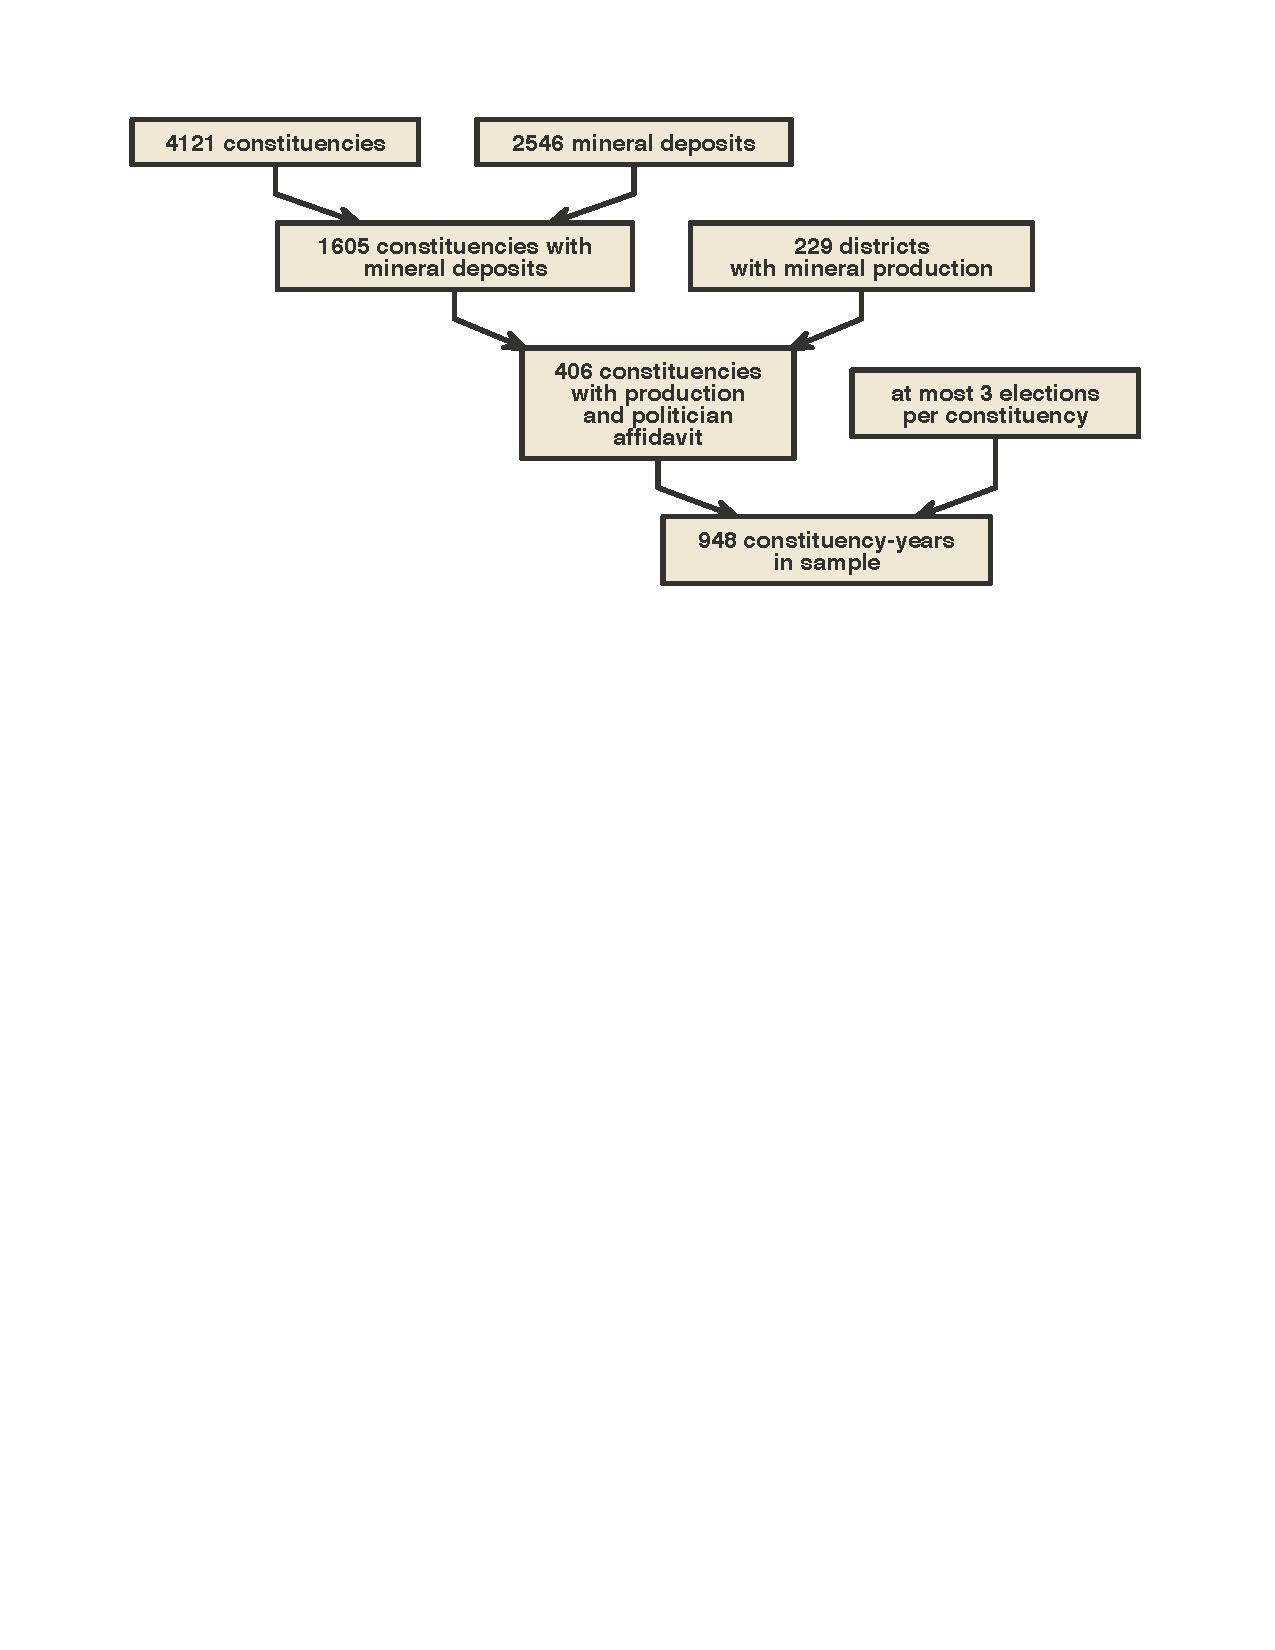
\includegraphics[scale=0.7]{\miningpath/nomnoml}
    \label{fig:app_sample}
  \end{center}
  \footnotesize{The figure describes the process for generating the
    sample of constituencies with valuable mineral deposits, based on
    predelimitation constituencies. The sample consists of 4121
    predelimitation constituencies. These are matched to 2546 mineral
    deposits (Geological Survey of India 2005), and to district-level
    production data (229 districts, Statistics of Mineral Information,
    Indian Bureau of Mines). 1605 constituencies are within 10km of
    mineral deposits, and 406 of these are in districts that report
    production of the same mineral between 1990 and 2013. Each
    constituency has either two or three elections in the sample
    period, leading to a main sample size in
    Table~\ref{tab:winner_crim} of 948 constituency-years.}
\end{figure}  


%%%%%%%%%%%%%%%%%%%%%%%%%%%%%%%%
%% SAMPLE CONSTRUCTION FIGURE %%
%%%%%%%%%%%%%%%%%%%%%%%%%%%%%%%%
\newpage
\begin{figure}[H]\caption{Moral Hazard Estimates: Robustness to Attrition}
  \begin{center}
    
    \small
    
    \textbf{Panel A: Log Asset Growth}
    
    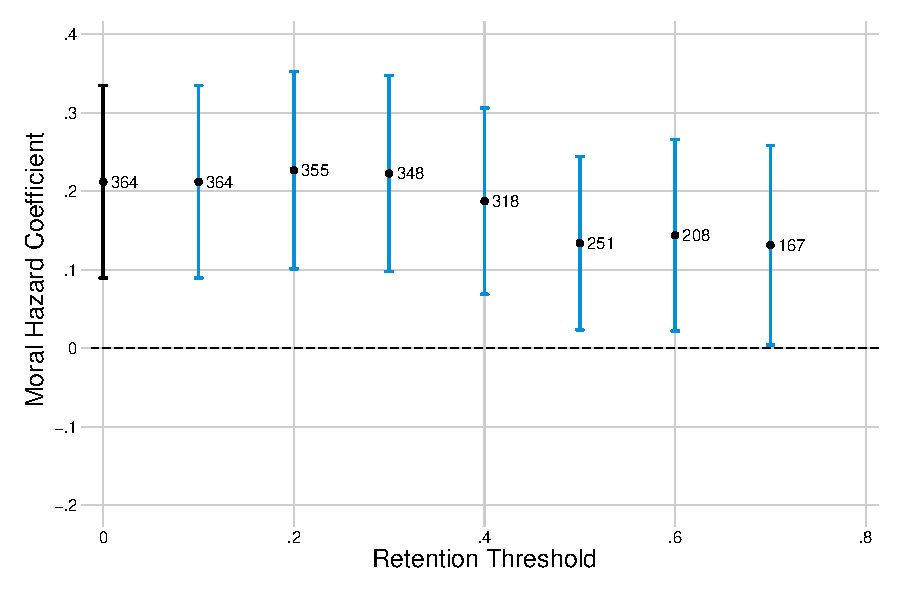
\includegraphics[scale=0.80]{\miningpath/mh_asset_robust}
    
    \label{fig:app_mh_attrition}

    \textbf{Panel B: Criminal Charge Growth}
    
    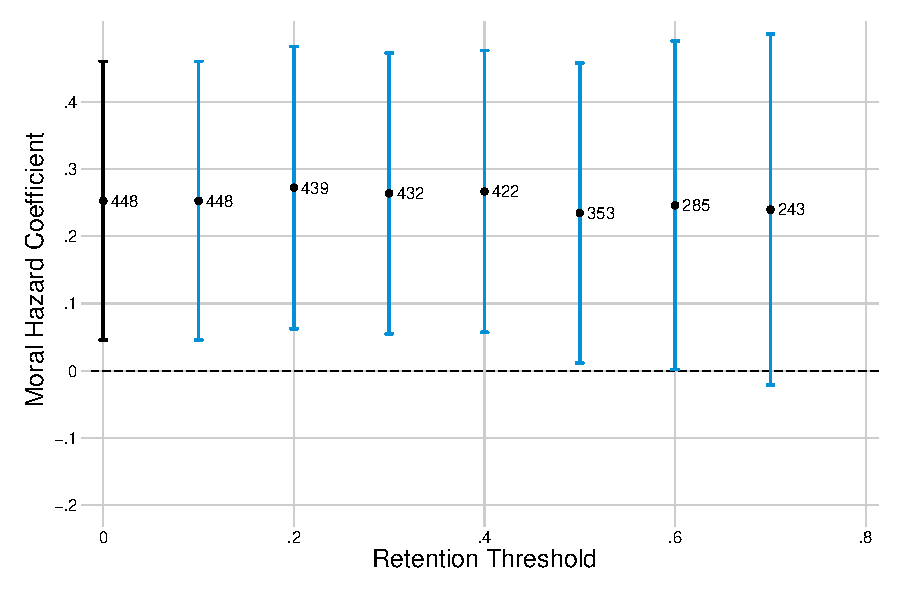
\includegraphics[scale=0.80]{\miningpath/mh_crime_robust}
    
  \end{center}
  \footnotesize{The figure shows alternate estimations of the moral
    hazard effects in Columns 1 and 4 of Table~\ref{tab:ts}. The
    retention threshold on the X axis is a state-election-level variable
    defined as the minimum share of constituencies in that election for which
    we were able to observe the winner again in the following
    election. The estimate at X=0 is the estimate in the paper. The
    remaining estimates increasingly shrink the sample to a set of
    elections where candidate attrition is less of a concern. The aim
    is to show the sensitivity of the estimates to potential
    attrition. The outcome variable is candidate change in
    assets in Panel A and change in criminal charges in Panel B. The
    regression estimate shows the effect of a change in local mineral
    wealth that occurs after an election on the change in assets or
    crime of the political representative serving that
    constituency. The points show the point estimate of each
    estimation along with the sample size.
  }
\end{figure}  


  
  \newpage
  %%%%%%%
  % MODEL
  %%%%%%%
  \section{Appendix For Online Publication: A Model of Collusion Between
    Firms and Politicians}
  \label{sec:model}
  \doublespacing

In this section, we present a political agency model to elucidate the
channels by which resource extraction operations influence the
behavior of politicians. The model is in the spirit of the career
concerns model of \citeasnoun{Persson2000}, which
\citeasnoun{Brollo2009} extend to allow endogenous entry of
politicians. Our model is oriented toward understanding rent-seeking
through illegal collusion between politicians and firms.

We focus on collusion between politicians and firms because that
relationship is suggested by the other literature on mining firms in
India and indeed in many other places around the world. Models of
politicians and firms have more commonly focused on the case where
politicians extract rents from firms to the detriment of those firms
\cite{Shleifer1994}. A model in that spirit would generate similar
predictions to those that we describe below, but it fits less well
with the qualitative evidence from India. Further, the facilitation of
black markets is widely associated in the literature with the presence
of violent actors
\cite{Tilly1985,Gambetta1996,Bandiera2003,Chimeli2011,Skarbek2011}.

We focus on two features of the resource extraction sector. First, the
mining sector generates rents, which can be expropriated by
politicians through their control over the regulatory inputs required
by mining firms. Second, mining is rife with illegality, both in India
and in other developing countries. This increases the dependence of
firms on local authorities, and raises the relative returns to both
politicians and firms willing to engage in illegal activity.
  
Consider a single mining firm that operates in a constituency
represented by a single politician. The mining operation has a high
fixed cost and a low marginal cost; the price of output is such that
the firm is profitable.  Politicians have a type that is characterized
by returns to illegal behavior $\theta \in (0,1)$. A high $\theta$
could represent a low risk aversion, indicating a willingness to risk
being caught and punished for crime. It could also represent a set of
skills that increase returns from criminal activities, such as a
propensity toward violence, or connections to criminal networks and
other corrupt officials.\footnote{We do not take a stand in the model
  on the relationship between $\theta$ and the politician's ability to
  provide services to constituents. \citeasnoun{Brollo2009} assume
  that corrupt politicians provide worse services to citizens;
  \citeasnoun{Vaishnav2017} argues they are better at providing
  services, in part because the formal state does such a poor job.}
Politicians who are caught in illegal activities pay a formal legal
punishment and may face worse odds of re-election.\footnote{While we
  view it as unlikely that voters would reward a politician for being
  convicted, the model only requires that the punishment from being
  caught outweighs any electoral benefit.}

We intentionally treat $\theta$ as a generally propensity toward crime
that is not specific to any type of crime, as this appears to fit the
context. Qualitative evidence suggests that a willingness to commit
crimes for one's party organization or local bosses is used as an
intentional signaling strategy. Such politicians may wish it to be
known that they are effective at acting outside of the law
\cite{Witsoe2009a,Berenschot2011a,Vaishnav2017}.

The model has two periods. In the first period, each candidate
chooses an election campaign effort level $e$, with a convex cost
$f(e)$. This could be a time cost or a financial cost. Election
outcomes cannot be predicted with certainty and the probability of
getting elected is a concave function of effort, which we denote
$\pi(e)$. The candidate's utility function is:

\begin{equation}
U = \pi(e)g(\cdot) - f(e)\text{,}
\end{equation}

\noindent where $g(\cdot)$ is the utility gain from getting
elected, and includes the continuation value of future elections.

In the second period, in exchange for payment, the elected politician
can take an illegal action that increases the firm's output, such as
granting an environmental clearance or land use permit that would have
been rejected by the formal process.\footnote{While the action itself
  may be legal or illegal, the exchange of the action for payment is
  illegal. Other actions could be expediting a permit that would have
  been granted anyway (a less serious crime), or arranging for police
  to arrest or intimidate local activists (a more serious crime).}
The action raises the firm's output by an increasing concave function
$q(a)$; more serious crimes (with higher $a$) have bigger effects on
output.\footnote{Any crimes for which the marginal profit is not
  increasing in the severity of the crime would be dominated choices,
  and thus not considered. We could model criminal competency by
  assuming that $q()$ is a positive function of $\theta$; this
  strengthens the predictions below because the politician trades off
  the increase in $q()$ against the cost of crime, which is decreasing
  in $\theta$.}  The action increases the firm's profit by $\mu q(a)$,
where $\mu$ is the mineral markup, or the difference between the price
and extraction cost of the mineral. If the politician takes the
illegal action, the rents are shared according to the Nash Bargaining
solution. We assume equal discount rates for simplicity but the model
results do not depend on this assumption, as long as the difference in
discount rates is not extreme.  The utility cost of illegal action is
$\frac{c(a)}{\theta}$, where $c()$ is a convex increasing function of
the severity of the action $a$.  The cost function encapsulates the
probability of being caught, the punishment conditional upon being
caught, and any future electoral consequences. High $\theta$
politicians pay a lower utility cost for committing a given crime.

Equation~\ref{eq:gain} summarizes the politician's net utility from
the illegal action:
%
\begin{equation}
\label{eq:gain}
g(a,\mu,\theta) = \frac{1}{2} \big(\mu q(a) - \frac{c(a)}{\theta}\big)\text{.}
\end{equation}

\noindent We solve the model by backward induction. In the second
period, the politician
chooses $a$ to maximize rents, trading off profit against the risk and
cost of
getting caught. The first order condition is:
%
\begin{equation}
\label{eq:foc1}
\mu q'(a^*)=\frac{c'(a^*)}{\theta}\text{.}
\end{equation}

\noindent Under Inada conditions, any politician with $\theta$ strictly greater
than zero will choose $a^* > 0$ and commit at least some illegal
action.\footnote{In the words of a four-time Chief Minister of Uttar
  Pradesh, ``Even an honest MLA [politician] gets a [10\%] kickback on
  discretionary spending'' \cite{Vaishnav2017}.}

If the price of mineral output, and thus the mineral markup $\mu$
rises, then crime severity $a^*$ must rise according to
Equation~\ref{eq:foc1}.\footnote{Specifically,
  $\frac{\partial{a^*}}{\partial{\mu}} =
  \frac{q'(a^*)}{\frac{c''(a^*)}{\theta}-\mu q''(a^*)}$.}
Since $\mu$ and $a^*$ are rising, the
politician's rents in Equation~\ref{eq:gain} must rise as
well.  This gives us the moral hazard result: when mineral rents are
high, politicians provide more illegal services to firms and both
firms and politicians earn greater rents from mining operations.

We now consider how politician type affects the effort exerted to
obtain office. Each candidate chooses an effort level such that the
marginal gain in terms of rents in office is equal to the marginal
cost of effort required to win:
%
\begin{equation}
f'(e^*) = \frac{1}{2} \pi'(e^*) \big( \mu q(a^*) - \frac{c(a^*)}{\theta}\big)\text{.}
\end{equation}
%
The change in effort in response to an increase in the mineral markup
is given by:
%
\begin{equation}
\frac{\partial e^*}{\partial \mu} = \frac{1}{2} \frac{\pi'(e^*)\cdot
  q(\mu,\theta)}{f''(e^*)-\pi''(e^*)\cdot g(\mu,\theta)}\text{.}
\end{equation}

\noindent The expression is positive. Politicians earn greater rents from office
when mineral rents are high, and therefore all candidates try
harder to win elections when mineral prices are high.
This has the biggest effect on effort when $q(\cdot)$ is large, and
thus when $\theta$ is large---that is, on the candidates with the
highest propensity toward illegal activity.  High mineral values will
increase the probability that a criminally inclined candidate gets
elected, unless the mineral shock also decreases voters' preferences
for criminal candidates. This is the adverse selection
effect.\footnote{For simplicity, we have assumed that mineral wealth
  does not affect voter preferences over candidate type. Voter
  preferences could shift in either direction. They may dislike
  criminal candidates, and pay closer attention to elections when
  rents are high, thus mitigating the adverse selection
  effect. Alternately, they may prefer criminal candidates if they are
  perceived to facilitate mining operations.  In the empirical part of
  this paper, we observe a joint outcome of voter preferences and
  candidate effort. The empirical test of the selection effect is thus
  jointly testing for the sum of the increase in candidate effort and
  any voter shift \textit{toward} the more criminal candidate.}  Both
the adverse selection and moral hazard effects lead to increased
illegal behavior by politicians in office when mineral rents are
high. These effects are likely not only additive, but reinforcing: the
moral hazard effect is worse for candidates who are more criminally
inclined. 

The model makes three key predictions, which we test in this
paper. First, positive mineral wealth shocks in the first period (i.e.
before elections take place) will lead criminal politicians to win
more elections. Second, positive mineral wealth shocks in the second
period (i.e. after candidates have been selected into office) will
cause politicians in office to gain wealth and commit more crimes. By
focusing on shocks that occur after candidates win elections, we can
thus isolate the moral hazard effect. Third, the wealth and crime
gains may occur for all types of politicians, but should be strongest
for the most criminal types.


\subsection{Modeling Electoral Fraud}
\label{app:model_fraud}

This subsection extends the model by considering the possibility that
politicians can use criminal activities or violence to win elections.

The structure is as before, but we assume that crime with the purpose
of winning elections, denoted by $a_e$, is distinctly chosen from
crime to increase mining output, which we call illegal mining and
denote by $a_m$. Both are punished with the same convex increasing
cost function $\frac{c(a)}{\theta}$. As above, we use backward
induction. We first solve for second period rents and criminal behavior
conditional on winning an election. Then, we solve for electoral
effort and electoral crime in the first period.

The elected politician earns the following rent, which is unchanged
from the model above:

\begin{equation}
g(a_m,\mu,\theta) = \frac{1}{2} \big(\mu q(a_m) -
\frac{c(a_m)}{\theta}\big)\text{.}
\end{equation}

The first order condition for the extent of illegal mining is unchanged:
\begin{equation}
\mu q'(a_m^*)=\frac{c'(a_m^*)}{\theta}\text{.}
\end{equation}

The politician's utility function is as follows. We add a
choice over electoral crime, and a cost function for electoral crime.

\begin{equation}
U = \pi(e,a_e)\frac{1}{2} \big(\mu q(a_m) -
\frac{c(a_m)}{\theta}\big) - f(e) - \frac{c(a_e)}{\theta}\text{.}
\end{equation}

As in the primary model, $e$ represents effort to win elections, $a_m$
is the extent of illegal mining, $\mu$ is the mineral markup, $q()$ is
the output from illegal mining activities,
$\theta$ is a measurement of propensity toward crime, and $f(e)$ is
the convex cost of electoral effort. We have added additional terms
$a_e$, which denotes the extent of electoral fraud, and $c(a_e)$, the
convex cost of electoral fraud, which incorporates both the
probability of getting caught and the utility punishment. The
probability of winning an election $\pi{e,a_e}$ now depends positively
on effort and electoral crime. This function is concave in both $e$
and $a_e$, and we assume for simplicity that the cross-partial
$\pi_{ea_e}$ is zero.\footnote{If the cross-partial is not zero, it is
  most likely positive, as investment in the capacity to commit one
  kind of crime (e.g. by hiring thugs or bribing police officers)
  likely lowers the cost of committing other crimes. A positive
  cross-partial derivative would further increase the adverse
  selection effect because it raises the return to electoral
  crime for politicians already involved in illegal mining.}

Candidates now jointly choose electoral effort and electoral
crime. The first order conditions are similar for these two choices,
but the amount of electoral crime depends directly on politician type:
\begin{equation}
\frac{\partial f}{\partial e^*} = \frac{1}{2} \frac{\partial \pi}{\partial e^*}
\big( \mu q(a_m^*) - \frac{c(a_m^*)}{\theta}\big)
\end{equation}


\begin{equation}
\frac{1}{\theta} \frac{\partial c}{\partial a_e^*} = \frac{1}{2} \frac{\partial
  \pi}{\partial a_e^*} \big( \mu q(a_m^*) -
\frac{c(a_m^*)}{\theta}\big)
\end{equation}

The moral hazard effect remains unchanged, because the decision about
how much illegal mining to facilitate happens only conditional upon
having been elected:

\begin{equation}
\frac{\partial a_m^*}{\partial \mu} =
\frac{q'(a_m^*)}{\frac{c''(a_m^*)}{\theta}-\mu q''(a_m^*)}
\end{equation}
\newline

There are now two adverse selection comparative statics. When the
mineral markup $\mu$ rises, candidates can change their effort levels,
and they can change their willingness to engage in electoral
crime. The expressions
for these comparative statics are calculated from the election effort
and crime first order conditions:

\begin{equation}
\frac{\partial e^*}{\partial \mu} = \frac{1}{2} \frac{\frac{\partial
    \pi}{\partial e^*}q(a_m^*)}{f''(e^*)-\frac{\partial^2\pi}{\partial e^*^2}
  g(a_m^*,\mu,\theta)}
\end{equation}

\begin{equation}
\frac{\partial a_e^*}{\partial \mu} = \frac{1}{2} \frac{\frac{\partial
    \pi}{\partial a_e^*} q(a_m^*)}{\frac{1}{\theta} \frac{\partial^2
    c}{\partial a_e^*^2} - \frac{ \partial^2 \pi}{\partial a_e^*^2}
  g(a_m^*,\mu,\theta)}
\end{equation}

The first expression is unchanged. The second expression demonstrates
a second form of adverse selection: mineral rents increase the return
to electoral crime, and do so especially for high $\theta$
politicians. This occurs because these politicians facilitate
more illegal mining $q(a_m^*)$ and thus have greater marginal returns
to crime when prices are high.

In conclusion, extending the model to give politicians the opportunity
to commit crimes to win elections strengthens the predictions on the
adverse selection effect.

  
\end{appendix}

\end{document}

